% Some commands used in this file

\chapter{Pre-Survey and Experiment Findings}
The following chapter will give an overview of the data obtained from the survey, which was conducted before running the experiment.
Later, an overview of the data obtained from the experiment is explained along with feedback received from the participants. This chapter puts forth
all that was learnt from the above mentioned.

\section{Overview of the Pre-Survey Data}
The survey has 199 participants. After filtering out spurious and half-filled entries 189 entries are used for the data analysis. In the following paragraphs we will presenting the information obtained in the survey.

Out of the total
participants 63.64\% are male and 36.36\% are female. The mean birth year was found to be 1985. The demographics of the participants is explained in the table \ref{tab:demo}. On the education level 2.53\% have not completed high school, 9.60\% have completed high school, 5.05\% have gone to some college, 28.79\% have obtained their bachelors degree, 39.90\% have gotten their masters degrees and 14.14\% have obtained their PHDs. About the employment of the participants 51.52\% are full time employees, 6.06\% are part time employed, 6.06\% are unemployed and looking for work, 1.52\% are unemployed and not looking for work, 0.51\% are retired and 41.92\% are students. None of the participants are disabled. 

Figure \ref{fig:pre_q6} depicts the various kinds of applications the population has on their mobile phones. As it can be seen, the most popular applications are social networking, transportation and music applications. Plot \ref{fig:pre_q7} shows the frequency of mobile usage among the population. It is observed that the majority of the people use their phones 36-70 times a day.

In figure \ref{fig:pre_q8}, the bars with the color dark blue represents for each level the percentage of participants. The scale of the levels are from one to five, one indicates that people do not care to five indicating that people care a lot about mobile sensor data. As observed, most people have answered level 3, meaning they care to a medium level and 77.28\% care to a level of 3 and above.

In the same figure, the color light blue shows the amount of contribution that sensors in general have in the data sharing decision. Level one indicates that it contributes none, level 5 means that it contributes a lot. It can be observed that most people find that sensors contribute to a level of 4. Similarly, the color green shows the amount of contribution stakeholders in general have in the data sharing decision. It can be observed that most people find that it contributed to a level of 4. Lastly, the color yellow depicts the level of contribution contexts have in the data sharing decision. Most people feel that it contributes to a level of 5.

From the above, it is understood that in general, more than the sensor, the more important thing in a data request is for what purpose the data is being collected followed by the entity to whom the data is traded with. The privacy intrusion levels of the participants for the individual different sensors, stakeholders and contexts has been explained in chapter \ref{exp}.

\begin{figure}[ht!]
\centering
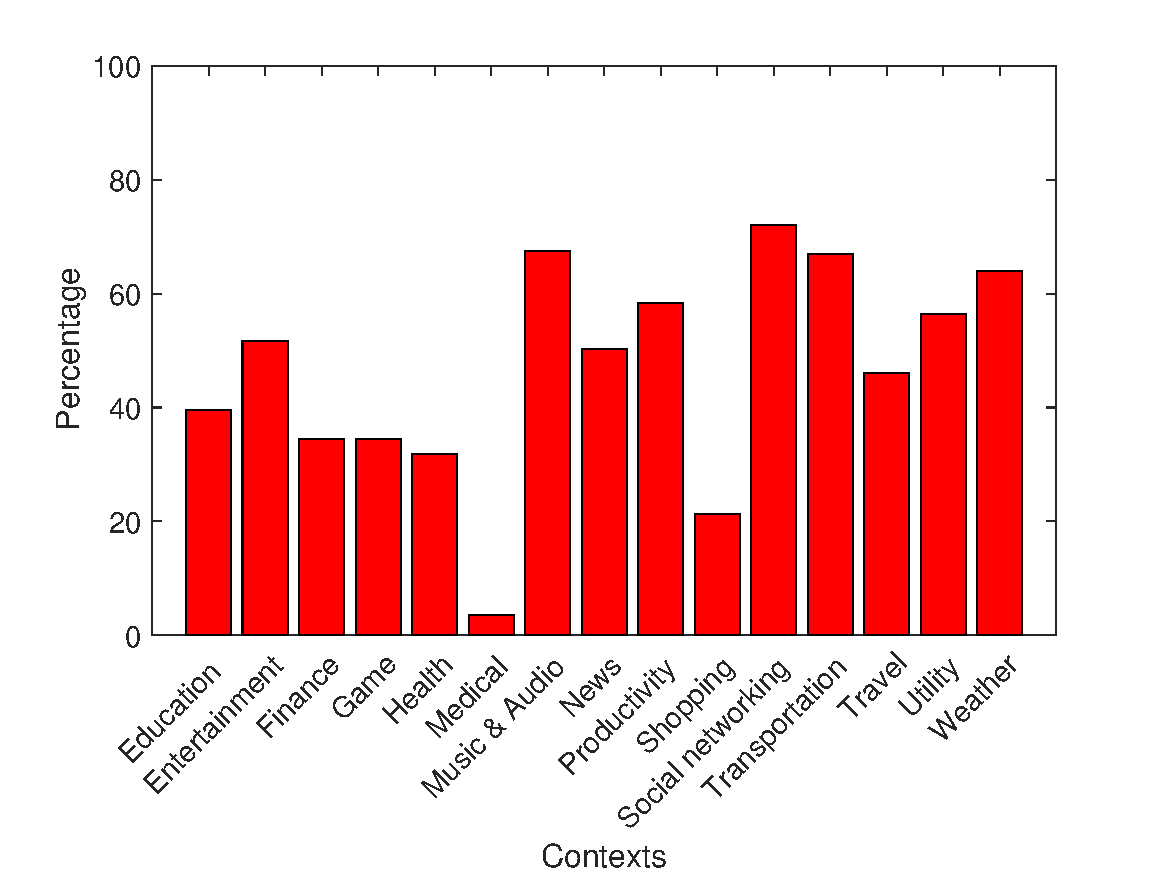
\includegraphics[width=\textwidth,keepaspectratio]{./images/pre_q6}
\caption{Applications in the Mobile Phone}
\label{fig:pre_q6}
\end{figure}

\begin{figure}[ht!]
\centering
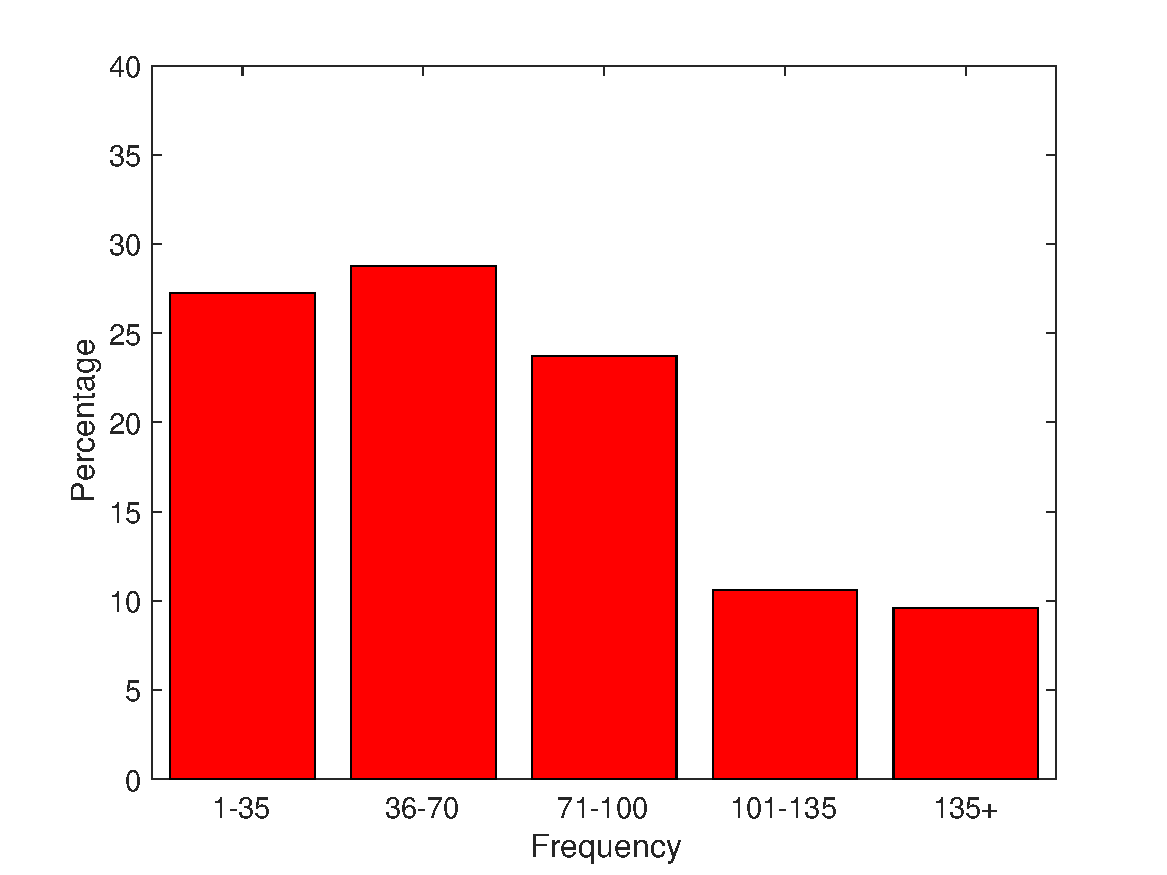
\includegraphics[width=\textwidth,keepaspectratio]{./images/pre_q7}
\caption{Frequency of Mobile Phone Usage}
\label{fig:pre_q7}
\end{figure}

\begin{figure}[ht!]
\centering
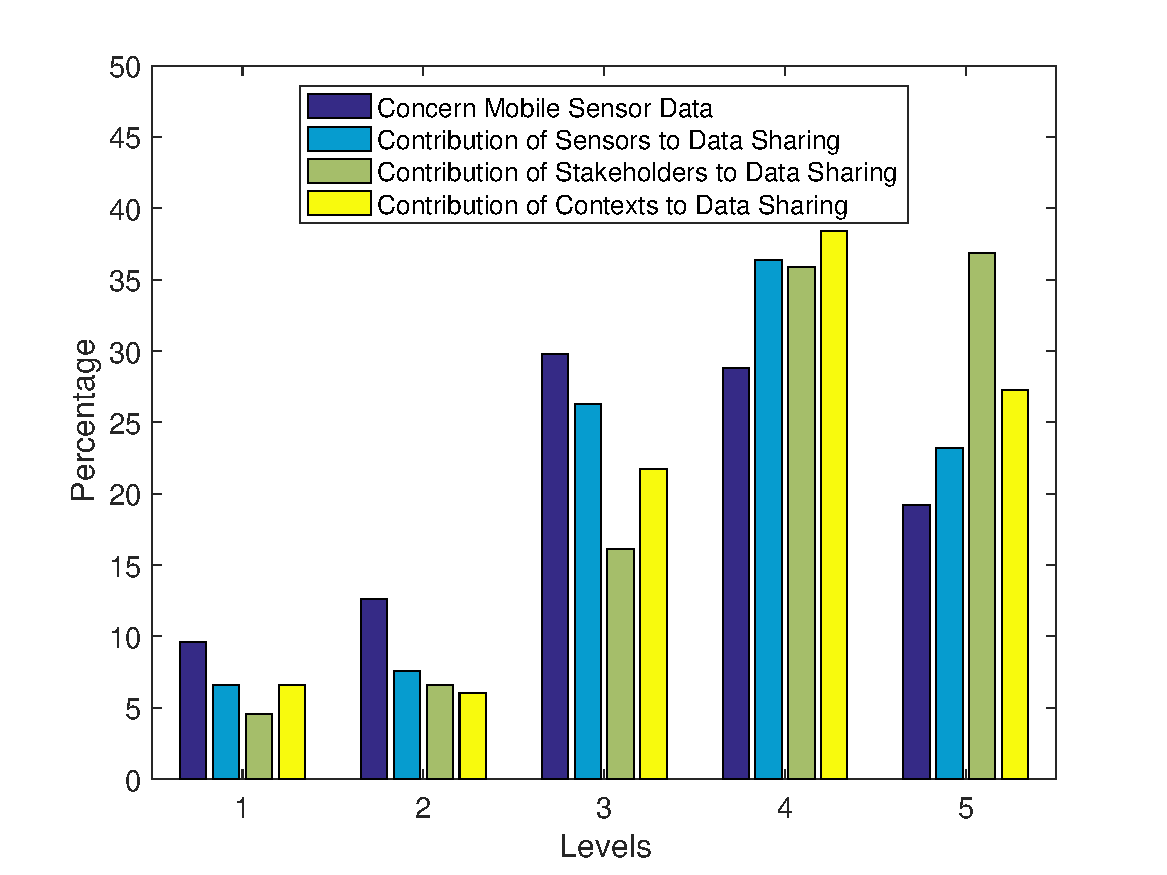
\includegraphics[width=\textwidth,keepaspectratio]{./images/pre_q8101214}
\caption{Graph depicting the concern of Mobile Sensor Data and the contribution of various features to the data sharing decision}
\label{fig:pre_q8}
\end{figure}

\begin{figure}[ht!]
\centering
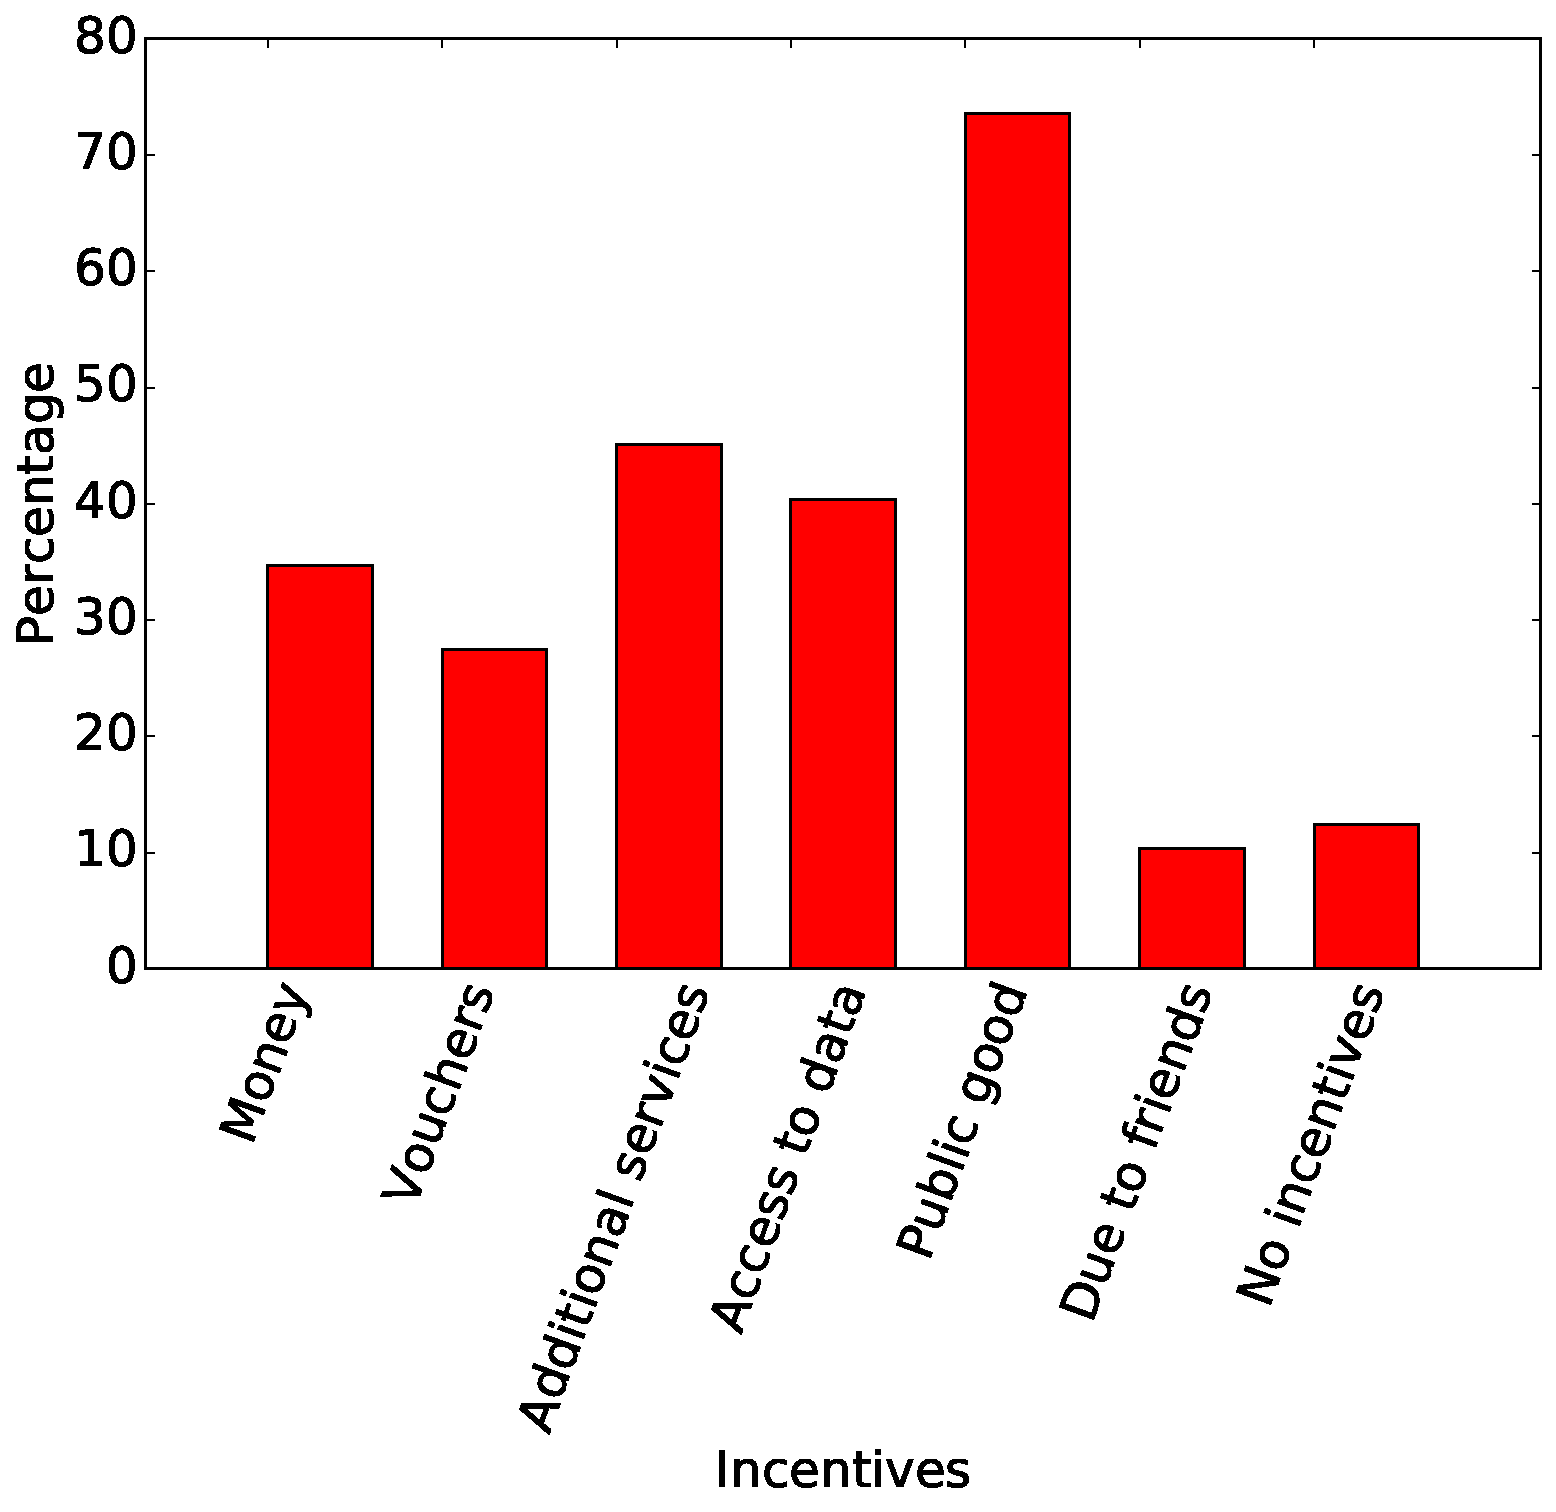
\includegraphics[width=\textwidth,keepaspectratio]{./images/pre_incentives}
\caption{Opinions on Incentives}
\label{fig:pre_q15}
\end{figure}

\begin{table}[h!]
  \centering
  \caption{Demographics of Population}
  \label{tab:demo}
  \begin{tabular}{cc}
    \toprule
     Country&Percentage\\
    \midrule
United States of America&1.01\%\\
United Arab Emirates&0.51\%\\
The former Yugoslav Republic of Macedonia&0.51\%\\
Syrian Arab Republic	&0.51\%\\
Switzerland&20.71\%\\
Spain	&1.01\%\\
Slovakia	&0.51\%\\
Serbia&	5.05\%\\
Russian Federation&	0.51\%\\
Netherlands	&1.52\%\\
Italy	&2.02\%\\
Iran&1.01\%\\
India	&14.65\%\\
Hungary	&0.51\%\\
Greece	&29.29\%\\
Germany	&10.61\%\\
France	&1.52\%\\
Czech Republic	&1.01\%\\
Costa Rica	&0.51\%\\
China	&0.51\%\\
Columbia	&0.51\%\\
Canada	&0.51\%\\
Bolivia	&0.51\%\\
Brazil	&1.52\%\\
Bahrain	&0.51\%\\
Argentina	&0.51\%\\
Austria & 2.02\%\\
    \bottomrule
  \end{tabular}
\end{table}

\section{Pre-Survey Methodology and Findings}
All the results presented below were performed on the data by performing the following changes to the data:
\begin{enumerate}
\item Rows with empty fields were removed
\item Rows with spurious data were removed
\item Data was scaled or normalized when necessary
\end{enumerate}

Other than the above, the data was not manipulated. Outliers were not excluded either.

\subsubsection{Perception of Individual Sensor Grouped on the Intrusion of Sensors in General}
We try to examine here if the perception of intrusion  of Sensors can affect the way a person views the individual sensors themselves. In other
words, we try to examine if there is a significant difference in perception of each sensor depending on the perception of the Sensors as a whole.
For this, we grouped the survey data based on the responses to question 10. Since there are 5 possible responses to this question, this makes 5 individual groups from 1 to 5.

We now have 5 groups who view sensors in a different light each and their perception of each of the individual sensors can be compared. Before going into the comparison, we try to understand the properties of the data. To perform a one-way ANOVA test or a t-test, the data needs to be:

\begin{enumerate}
\item Normally distributed
\item Homoscedastic
\item Ordinal or continuous
\end{enumerate}

Since the data is discrete and follows the Likert Scale with options from 1 to 5, it gives skewed normal distribution. Additionally, the variances of values within the groups formed are not similar. One-way ANOVA test is quite robust to heteroscedacity, as long as the maximum variance among all groups is less than four times the group with the lowest variance. The scale used to collect data is in the ordinal form. Accounting for all the violations, we instead opt for a non-parametric tests such as the Kruskal-Wallis H test and the Dunn's test
which only assume the following : 

\begin{enumerate}
\item Groups are independant from one another
\item All observations are independant
\item The dependant variables should be in the ordinal scale or continuous
\end{enumerate}

The above tests do not make any assumptions about the distribution of the data and are robust to heteroscedastic data.
\begin{figure}[htp]
\subtop[Mean of each Group for each Sensor\label{fig:s1}]{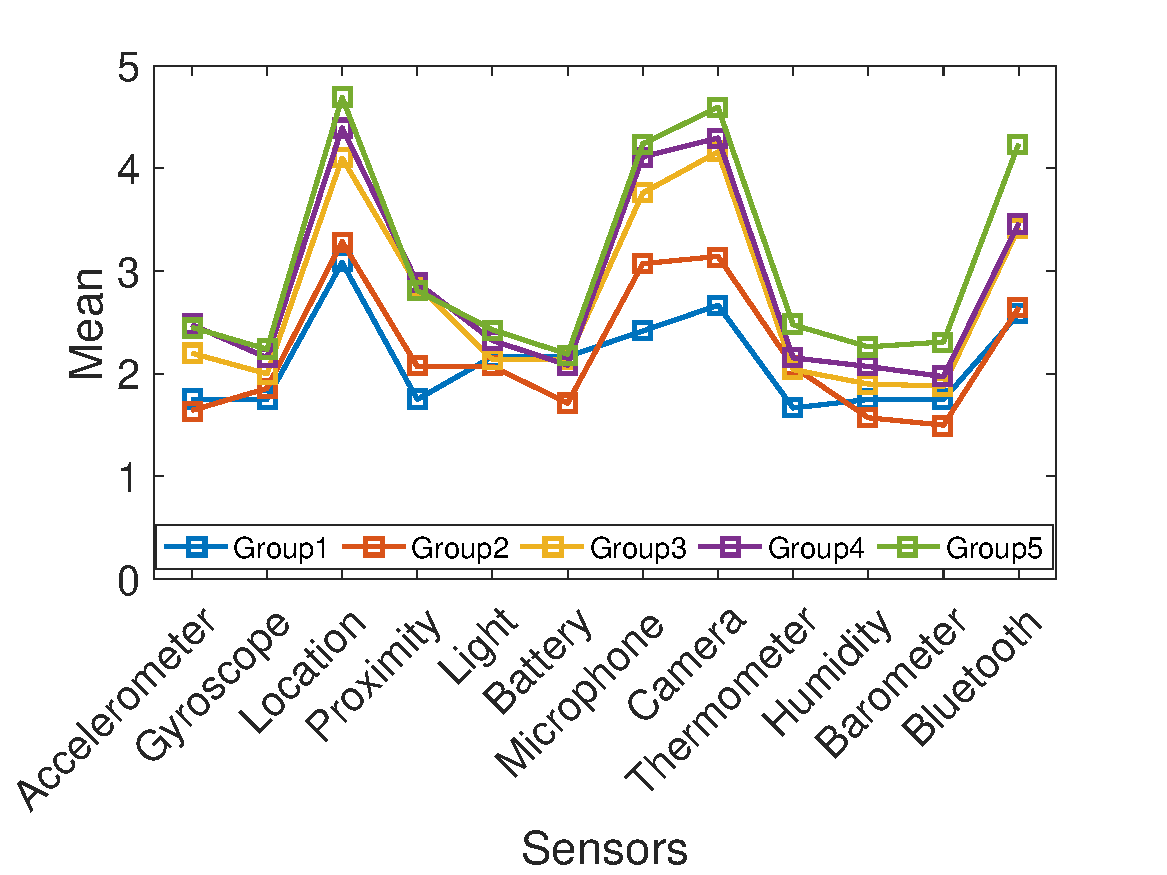
\includegraphics[width=0.5\linewidth]{./images/sensors_group_meanQ10}}
\subtop[Variance of each Group for each Sensor\label{fig:s2}]{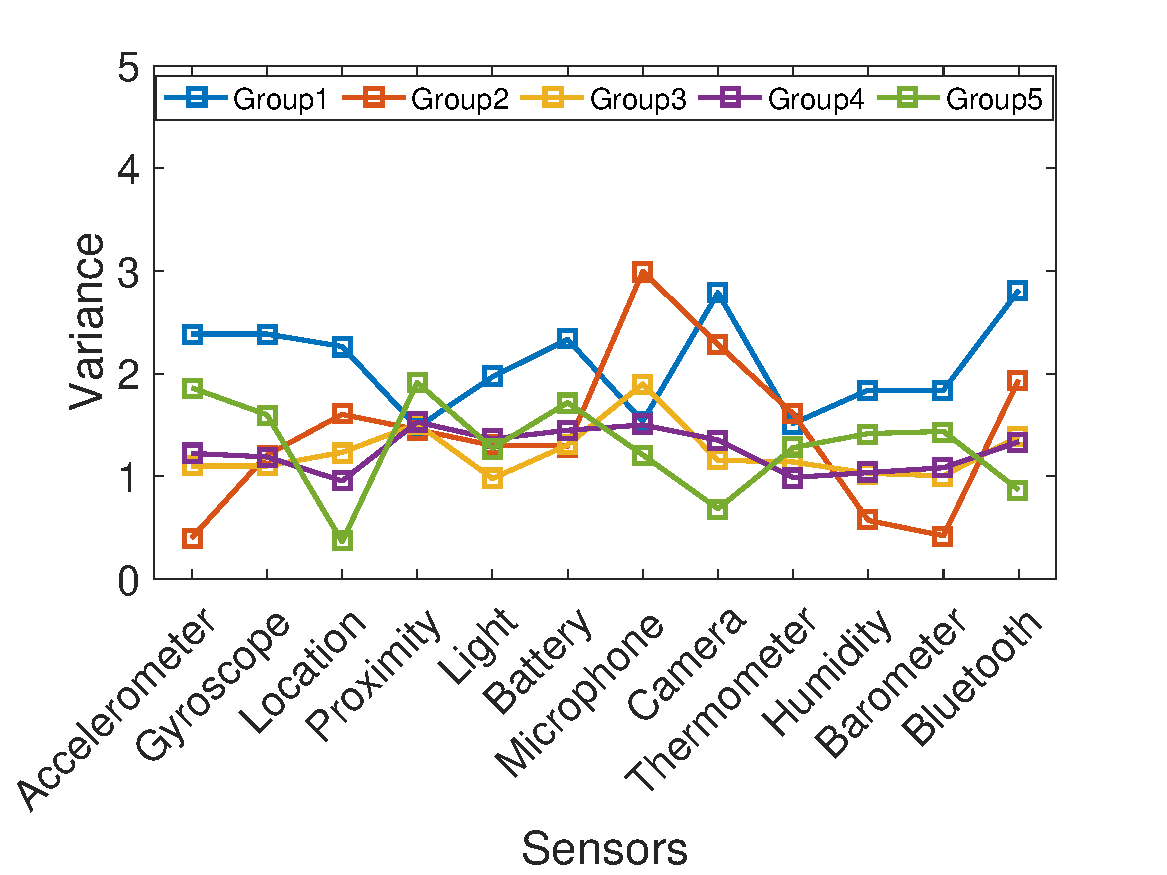
\includegraphics[width=0.5\linewidth]{./images/sensors_group_varianceQ10}}
\caption{Table Schemas}
\label{fig:s3}
\end{figure}

Group 1 to 5 have 13, 14, 50, 71 and 42 people each respectively. For in depth analysis of the composition of each group in terms of employment, education, gender and birth year please refer to tables
\ref{tab:emp_sensors},\ref{tab:edu_sensors},\ref{tab:gender_sensors},\ref{tab:year_sensors}. Figures \ref{fig:s1} and \ref{fig:s2} depict the mean and variances for each of the individual groups. We start by performing the non paramteric Kruskal-Wallis test on each Sensor. The value of alpha assumed here is 0.05. The null hypothesis states that all the groups perceive the sensors in the similar way. This means they come from the same distribution. The alternative hypothesis is
that the groups perceive each sensor in a significantly different way. The table \ref{tab:kw_sensors} depicts the p-values obtained from the test.


\begin{table}[h!]
  \centering
  \caption{Employment Classification of Groups}
  \label{tab:emp_sensors}
  \begin{tabular}{cccccc}
    \toprule
     Occupation&1&2&3&4&5\\
    \midrule
Employed full time&4.90\%&6.86\%&26.47\%&38.24\%&23.53\%\\
Employed part time&8.33\%&16.67\%&33.33\%&16.67\%&25.00\%\\
Unemployed and looking for work&8.33\%&16.67\%&16.67\%&25.00\%&33.33\%\\
Unemployed and not looking for work&0.00\%&0.00\%&0.00\%&66.67\%&33.33\%\\
Retired&0.00\%&0.00\%&100.00\%&0.00\%&0.00\%\\
Student&7.23\%&4.82\%&26.51\%&39.76\%&21.69\%\\
Disabled&0.00\%&0.00\%&0.00\%&0.00\%&0.00\%\\
    \bottomrule
  \end{tabular}
\end{table}



\begin{table}[h!]
  \centering
  \caption{Gender Classification of Groups}
  \label{tab:gender_sensors}
  \begin{tabular}{cccccc}
    \toprule
     Gender&1&2&3&4&5 \\
    \midrule
Female&5.56\%&4.17\%&33.33\%&30.56\%&26.39\% \\
Male&7.14\%&9.52\%&22.22\%&39.68\%&21.43\% \\
    \bottomrule
  \end{tabular}
\end{table}



\begin{table}[h!]
  \centering
  \caption{Average Birth Year of Groups}
  \label{tab:year_sensors}
  \begin{tabular}{ccccc}
    \toprule
     1&2&3&4&5\\
    \midrule
	1989& 1979& 1986& 1986& 1983\\
    \bottomrule
  \end{tabular}
\end{table}


\begin{table}[h!]
  \centering
  \caption{Education Classification of Groups}
  \label{tab:edu_sensors}
  \begin{tabular}{cccccc}
    \toprule
     Education&1&2&3&4&5\\
    \midrule
    
Less than high school&20.00\%&20.00\%&20.00\%&40.00\%&0.00\%\\
High school&10.53\%&0.00\%&52.63\%&31.58\%&5.26\%\\
Some college&10.00\%&20.00\%&30.00\%&20.00\%&20.00\%\\
Bachelors degree&7.02\%&10.53\%&24.56\%&42.11\%&15.79\%\\
Masters degree&3.80\%&5.06\%&24.05\%&35.44\%&31.65\%\\
PhD degree&7.14\%&7.14\%&17.86\%&35.71\%&32.14\%\\
    \bottomrule
  \end{tabular}
\end{table}  




\begin{table}[h!]
  \centering
  \caption{Kuskal-Wallis Test}
  \label{tab:kw_sensors}
  \begin{tabular}{cccc}
    \toprule
     Sensor & p-value \\
    \midrule
    Accelerometer & 0.0151 \\
    Gyroscope & 0.2959\\
    Location & 1.0664e-05\\
    Proximity & 0.0147\\ 
    Light & 0.6933\\
    Battery & 0.6950\\ 
    Microphone & 3.0070e-04\\
    Camera & 2.1191e-05\\
    Thermometer & 0.0693\\ 
    Air Humidity & 0.1292\\
    Barometer & 0.0949\\
    Bluetooth & 3.4877e-05\\ 
    \bottomrule
  \end{tabular}
\end{table} 

On these sensors, we proceed with a post hoc test by performing a pariwise Dunn's test to examine if there is an actual significant difference between the groups and if so between which groups. The sensors with p values with less than 0.05 are examined in more detail and the p-values are presented in table \ref{tab:dunn_sensors}. The table shows the results for each pairwise test done, with the p-values adjusted using the Bonferroni Method. The reason for choosing to adjust the p-values is that repeated experiments can increase the chances of accepting the alternative hypothesis so p-values are adjusted according to the number of experiments performed. 10 experiments are performed per sensor.

\begin{table}[h!]
  \centering
  \caption{Dunn's Test 1}
  \label{tab:dunn_sensors}
  \begin{tabular}{ccccccc}
    \toprule
     Groups & Accelerometer & Location & Proximity & Microphone & Camera & Bluetooh \\
    \midrule
    (1,2) & 1.0000 & 1.0000 & 0.9992 & 0.8365 & 1.0000 & 1.0000 \\
    (1,3) & 0.4207 & 0.2084 & 0.0699 & 0.0365 & 0.0732 & 0.7825 \\
    (1,4) & 0.0595 & 0.0125 & 0.0513 & 0.0012 & 0.0048 & 0.6442 \\
    (1,5) & 0.2054 & 0.0010 & 0.1191 & 0.0009 & 0.0007 & 0.0029 \\
    (2,3) & 0.6548 & 0.1774 & 0.3713 & 0.8927 & 0.1694 & 0.5921 \\
    (2,4) & 0.1185 & 0.0077 & 0.2617 & 0.2287 & 0.0123 & 0.4270 \\
    (2,5) & 0.3659 & 0.0005 & 0.5184 & 0.1597 & 0.0018 & 0.0007 \\
    (3,4) & 0.8989 & 0.7642 & 1.0000 & 0.8052 & 0.9040 & 1.0000 \\
    (3,5) & 0.9997 & 0.0869 & 1.0000 & 0.6390 & 0.2947 & 0.0066 \\
    (4,5) & 0.9998 & 0.8360 & 1.0000 & 1.0000 & 0.9617 & 0.0059 \\
    \bottomrule
  \end{tabular}
\end{table} 

\begin{figure}[htp]
\subtop[Mean of each Group for each Stakeholder\label{fig:st1}]{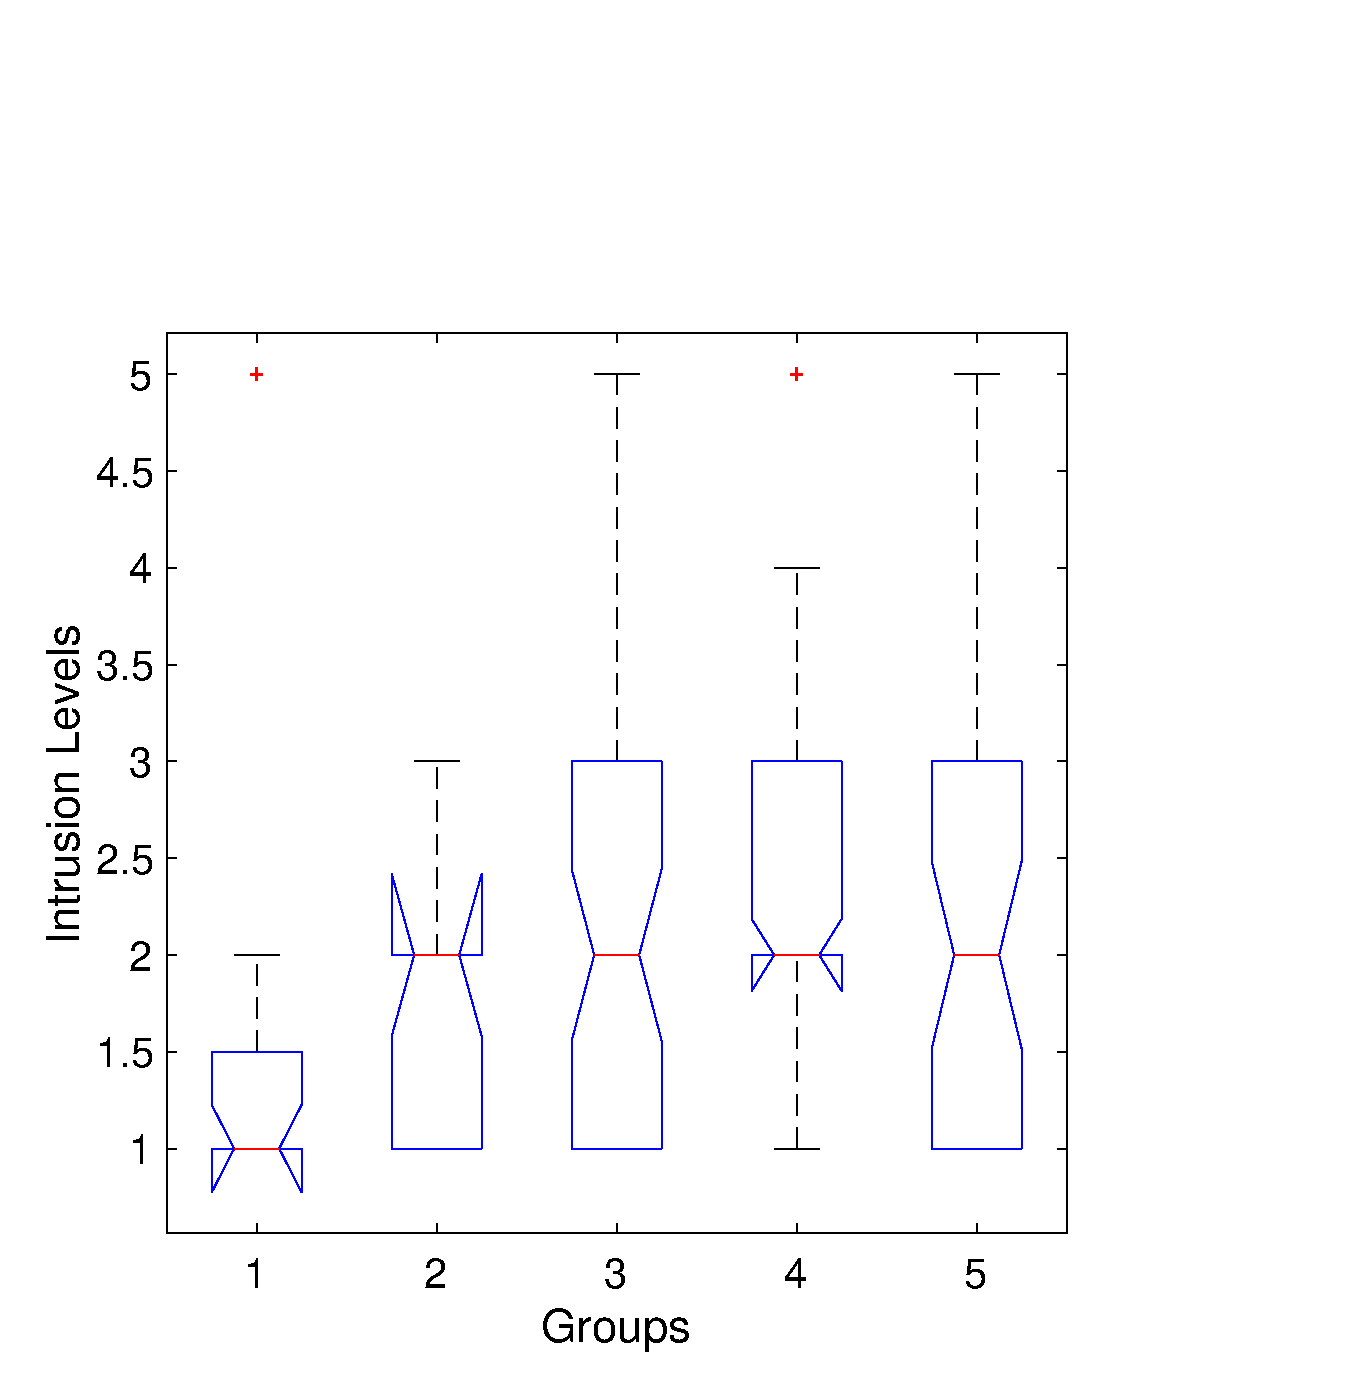
\includegraphics[width=0.4\linewidth]{./images/acc_box}}\hspace{1em}
\subtop[Variance of each Group for each Stakeholder\label{fig:st2}]{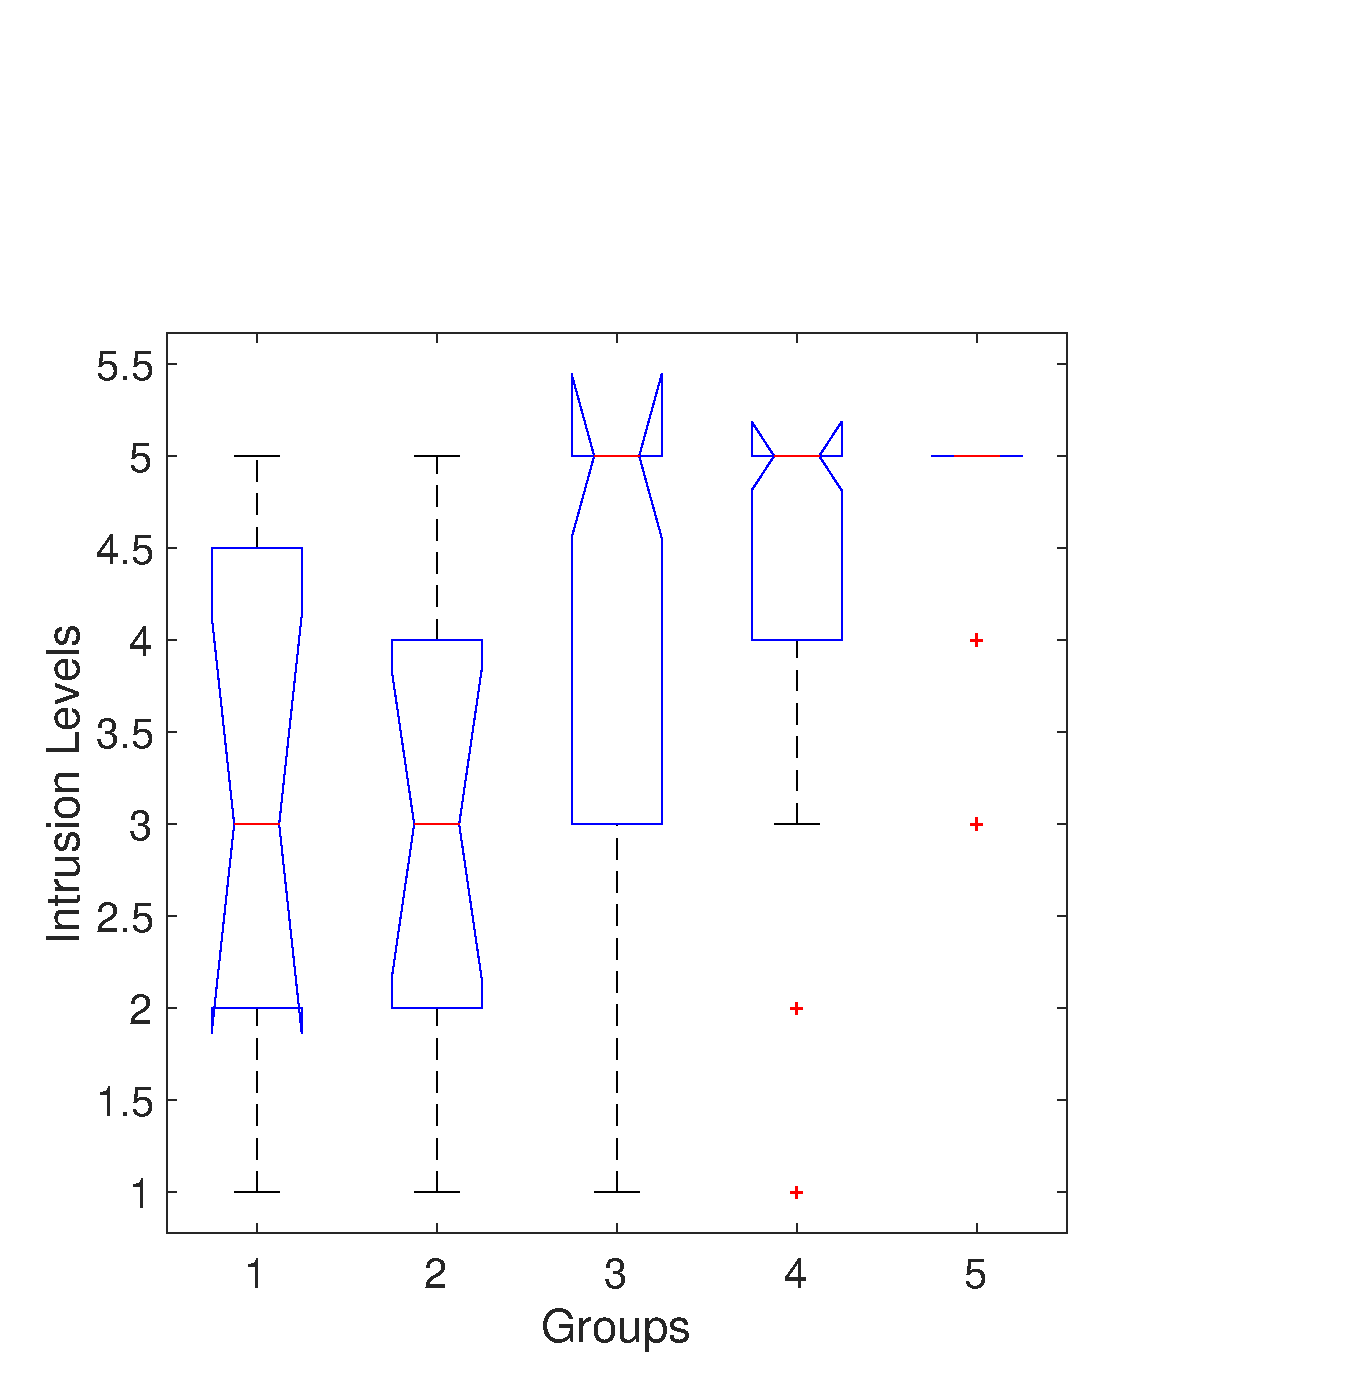
\includegraphics[width=0.4\linewidth]{./images/loc_box}} \newline
\subtop[Variance of each Group for each Stakeholder\label{fig:st5}]{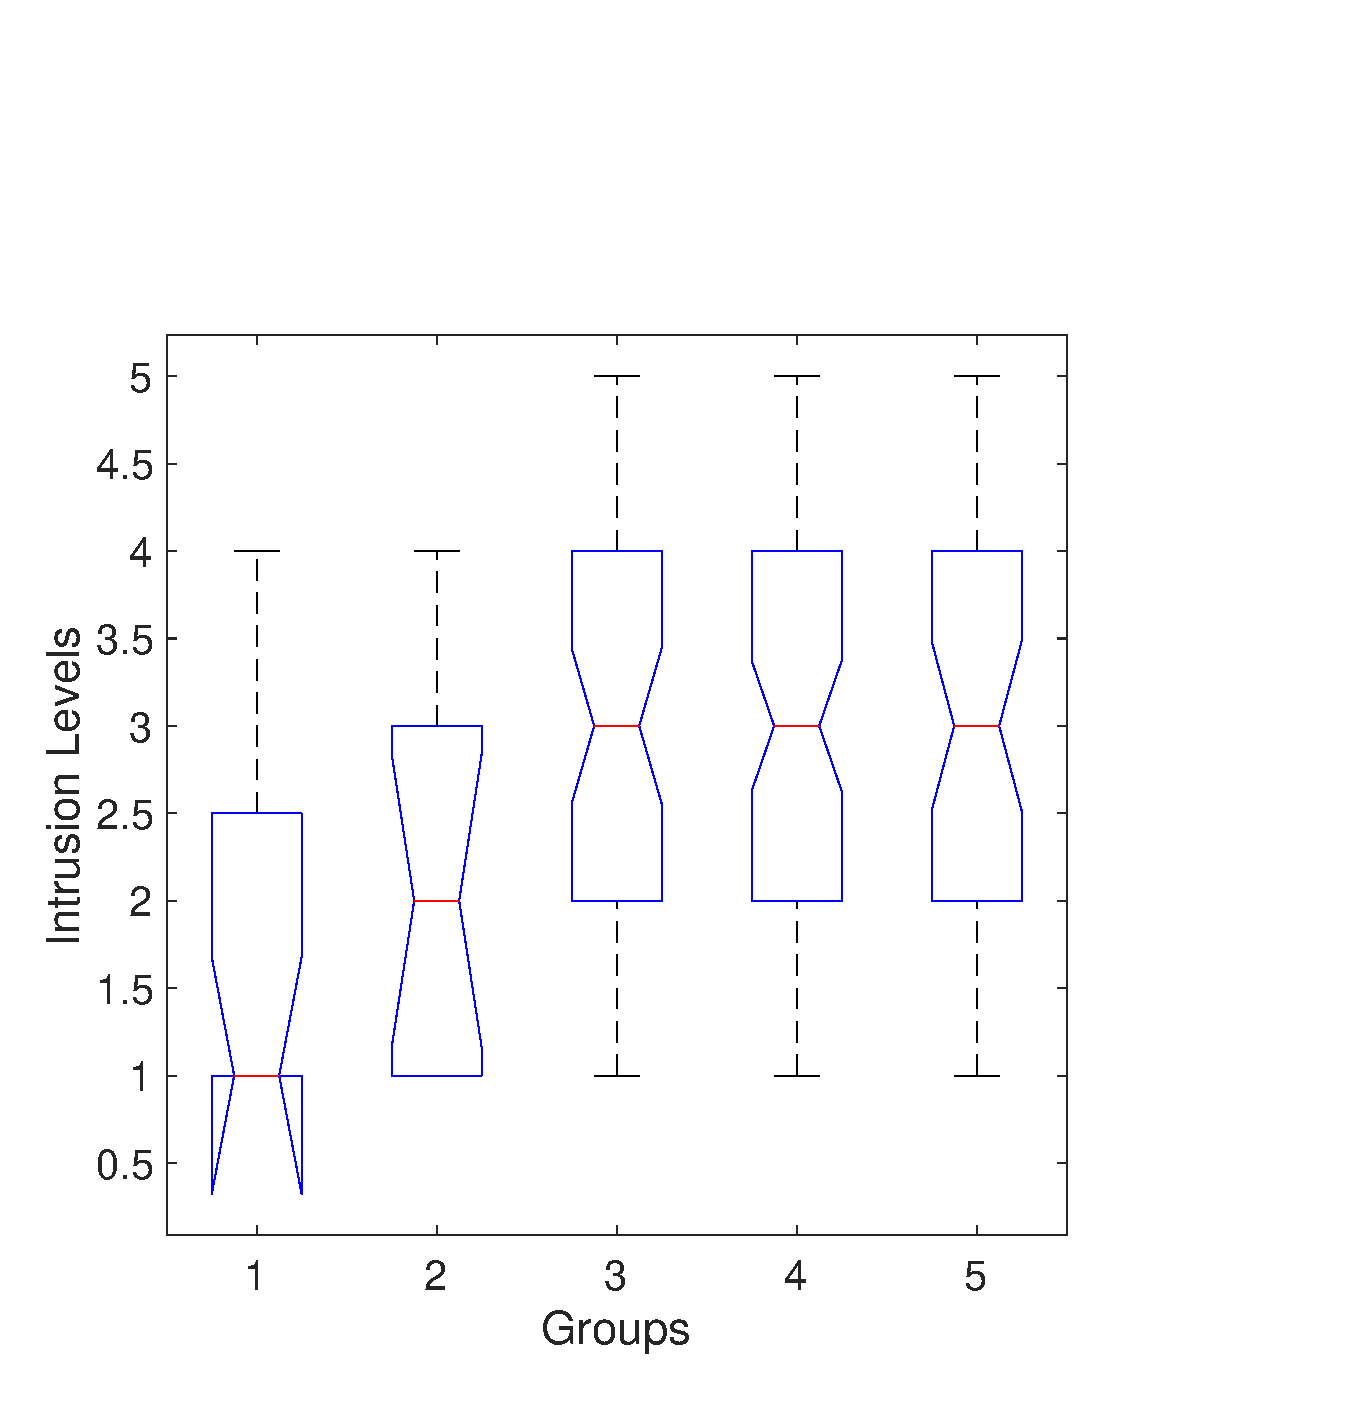
\includegraphics[width=0.4\linewidth]{./images/prox_box}}\hspace{1em}
\subtop[Variance of each Group for each Stakeholder\label{fig:st2}]{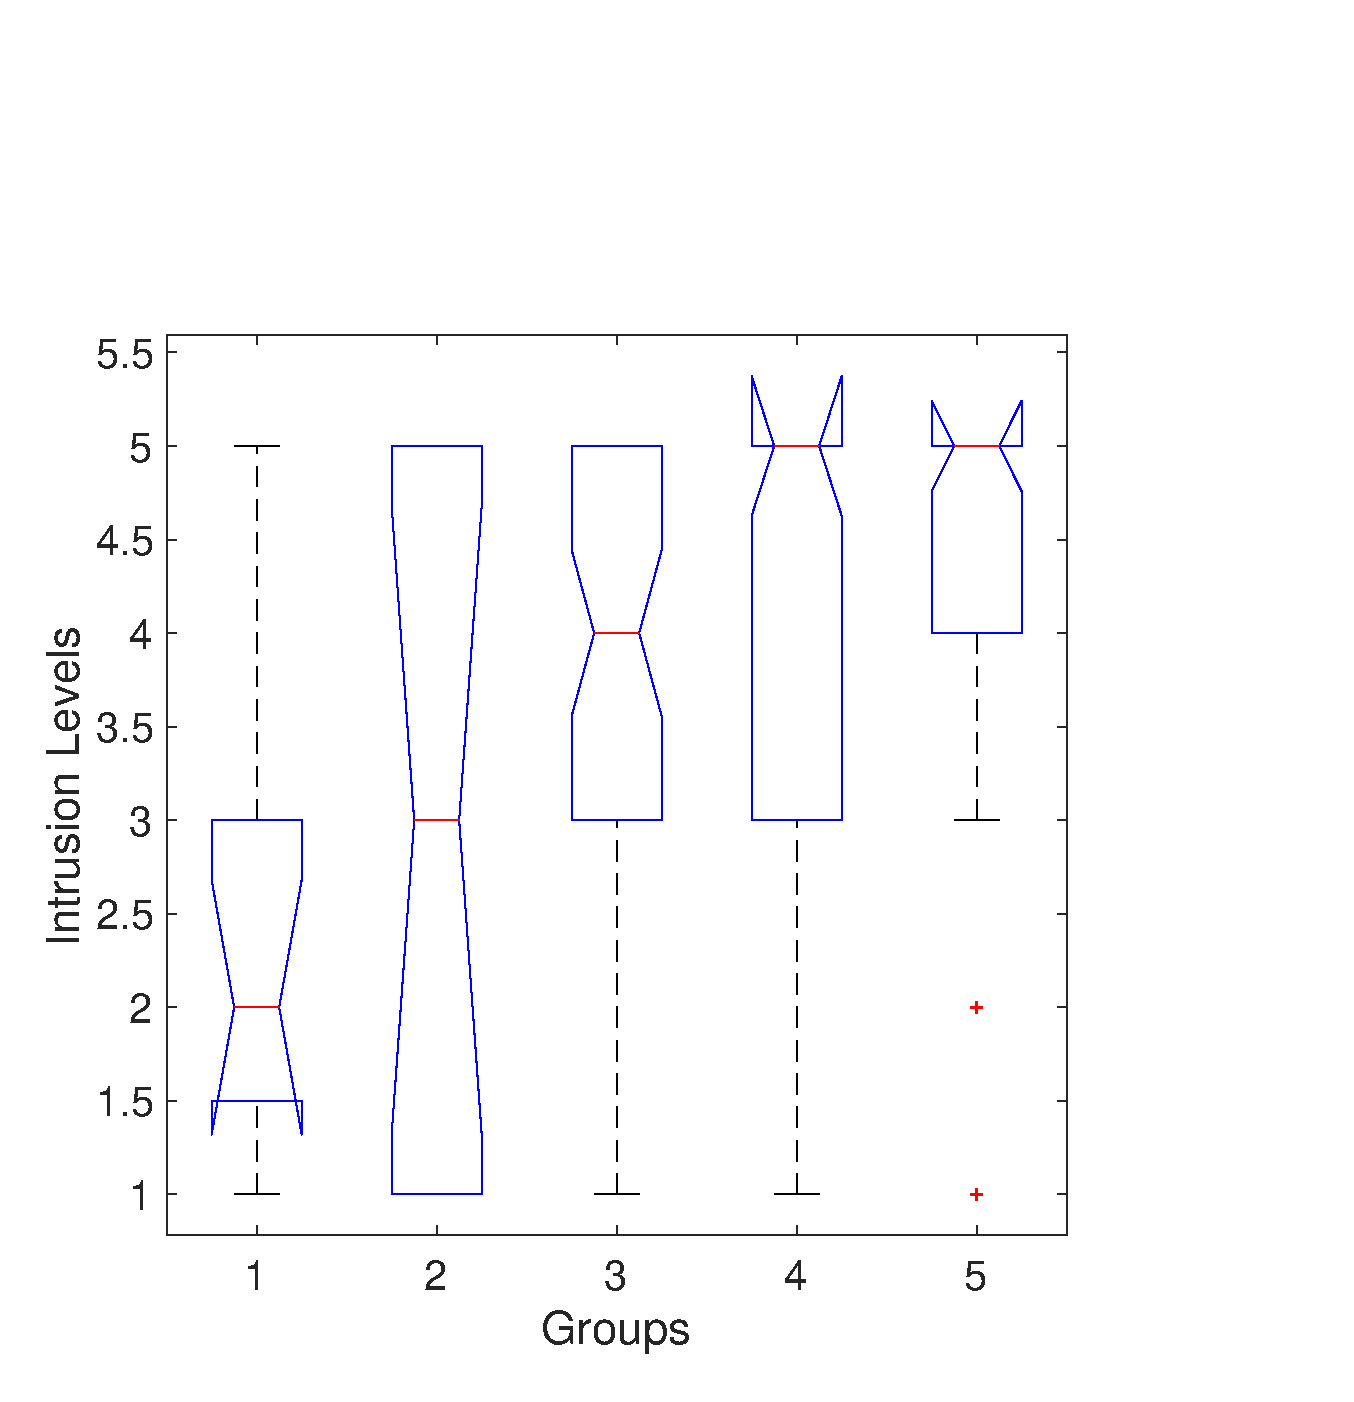
\includegraphics[width=0.4\linewidth]{./images/micro_box}} \newline
\subtop[Variance of each Group for each Stakeholder\label{fig:st5}]{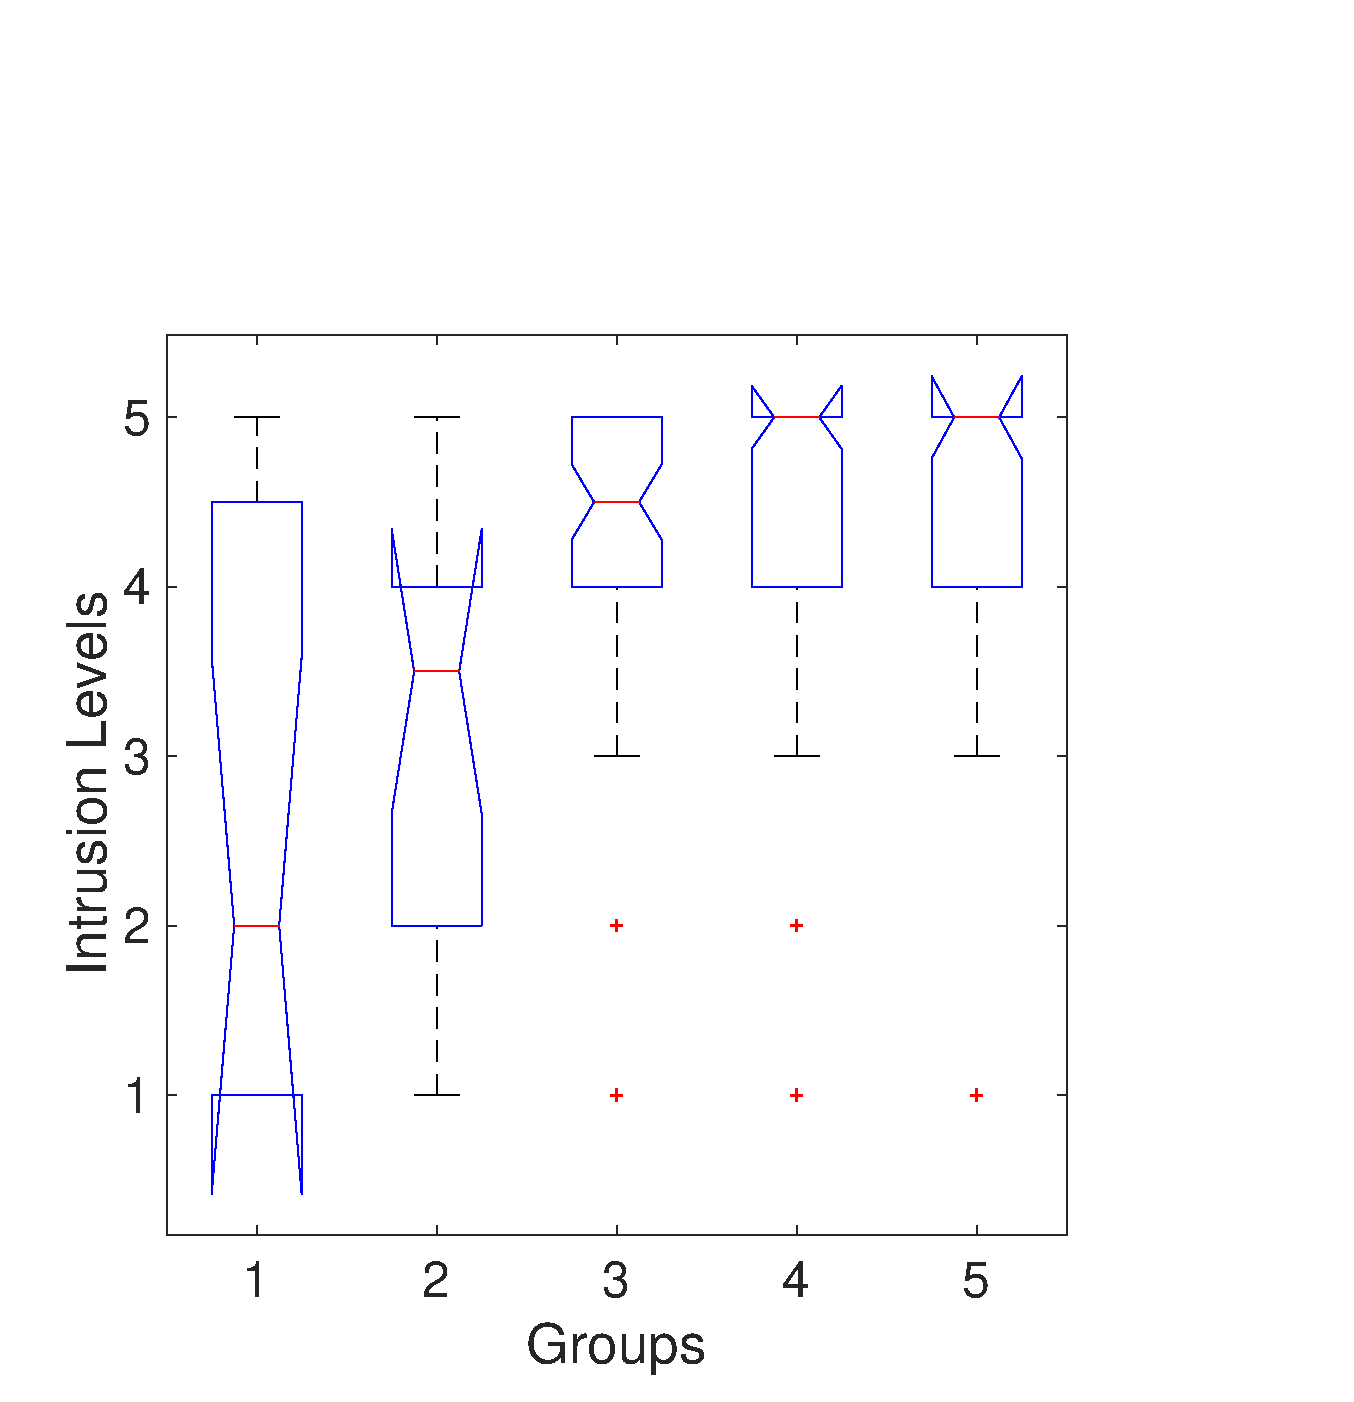
\includegraphics[width=0.4\linewidth]{./images/camera_box}}\hspace{1em}
\subtop[Variance of each Group for each Stakeholder\label{fig:st2}]{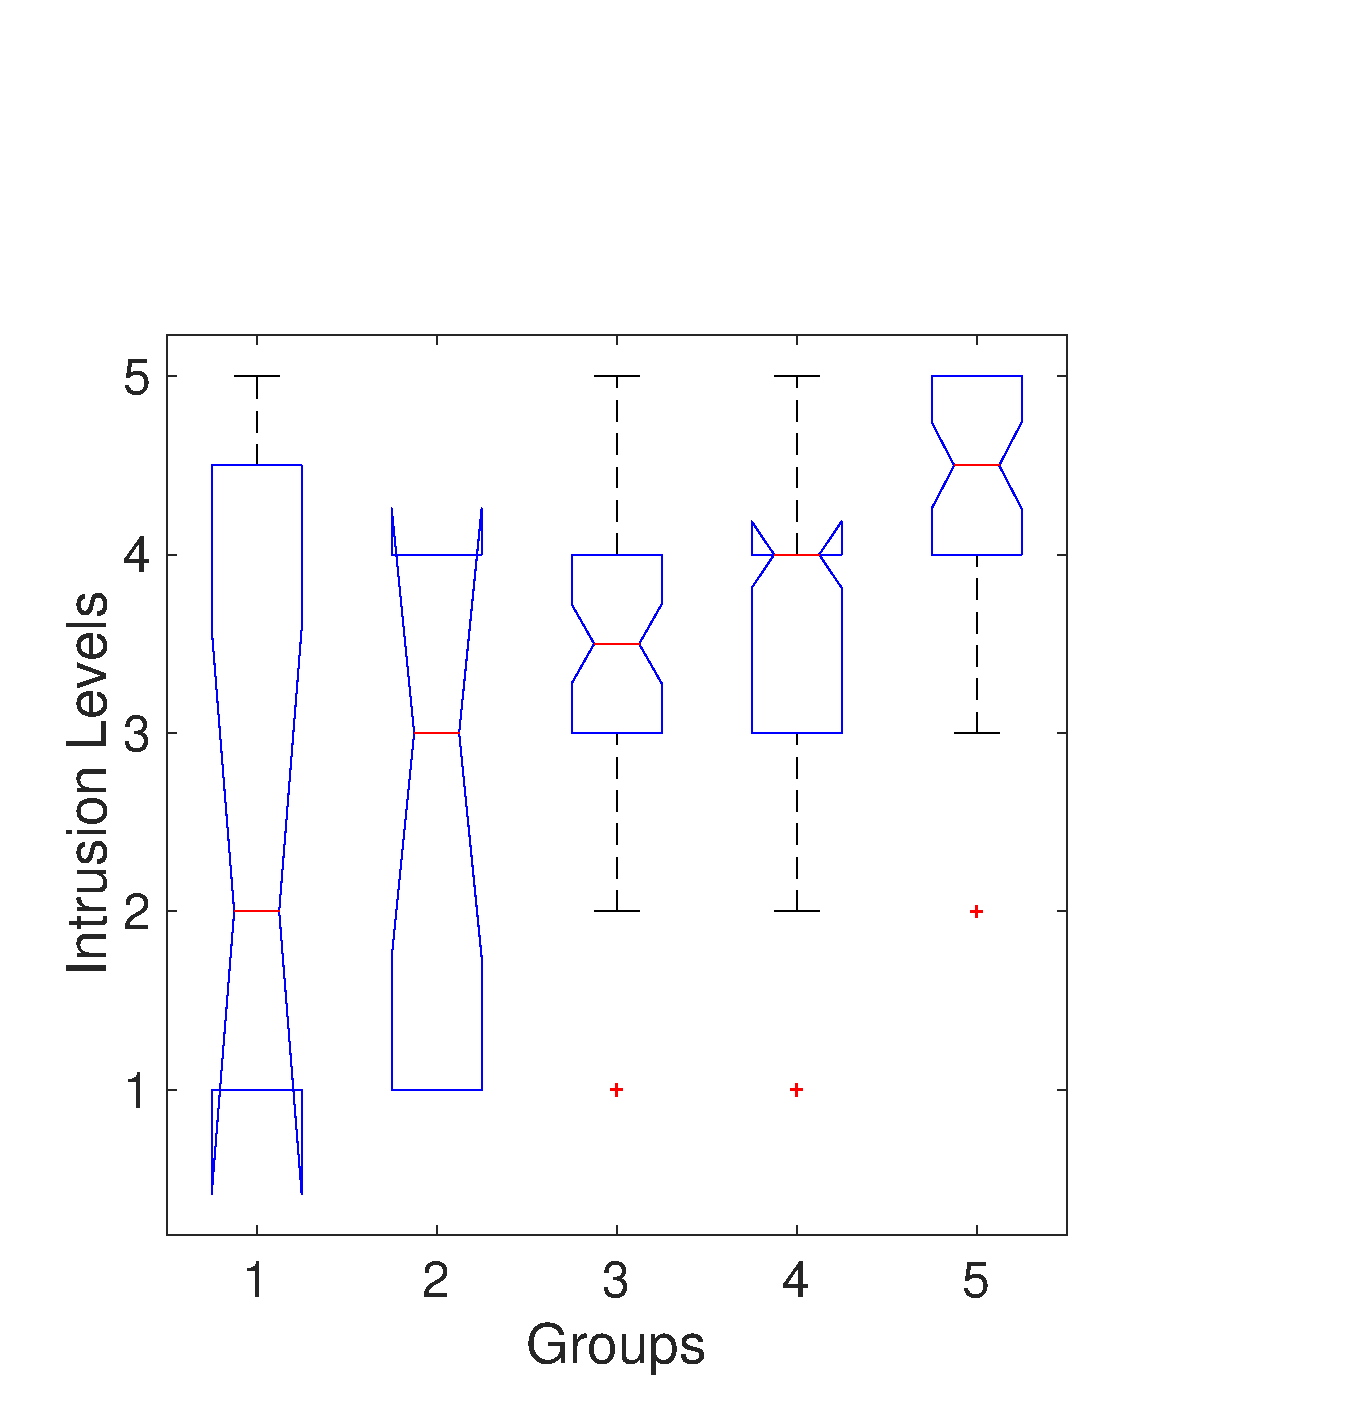
\includegraphics[width=0.4\linewidth]{./images/blue_box}}
\caption{Table Schemas}
\label{fig:st3}
\end{figure}



For the Accelerometer and Proximity, we can see that none of the pairwise groups have a significant difference from each other. This means that even tough the groups perceive sensors differently in general, they all view Accelerometers and Proximity in a similar way. 

For the location sensor, it can be observed that groups (1,4), (1,5), (2,4), (2,5) have a significant difference. This can be attributed to the fact that since the groups are formed from the perception of people of the Sensors Feature, the difference in perception between group 1 and group 5 will be larger than between group 1, group 2 and group 1, group 3 since they are not much apart in the scale.

For the microphone sensor, it can be seen that groups (1,3), (1,4) and (1,5) are significantly different from each other. This goes to show that
if people rate sensors as even a little intrusive, they all rate the microphone's in a significantly different way than the people who rate sensors as non-intrusive.

For the camera sensor, it can be observed that groups (1,4), (1,5), (2,4), (2,5) have a significant difference in their perception of the intrusion.
Similar to the location sensor, people with perception of sensors in general with a lower intrusion level have significantly different responses to the camera intrusion than the people who rate sensors with more intrusion.

For the Bluetooth sensor, there is a significant difference between groups (1,5), (2,5), (3,5) and (4,5). This shows that responses by people who find sensors extremely intrusive is different from the rest of the groups.


\subsubsection{Perception of Individual Stakeholders Grouped on the Intrusion of Stakeholders in General}

\begin{figure}[htp]
\subtop[Mean of each Group for each Stakeholder\label{fig:st1}]{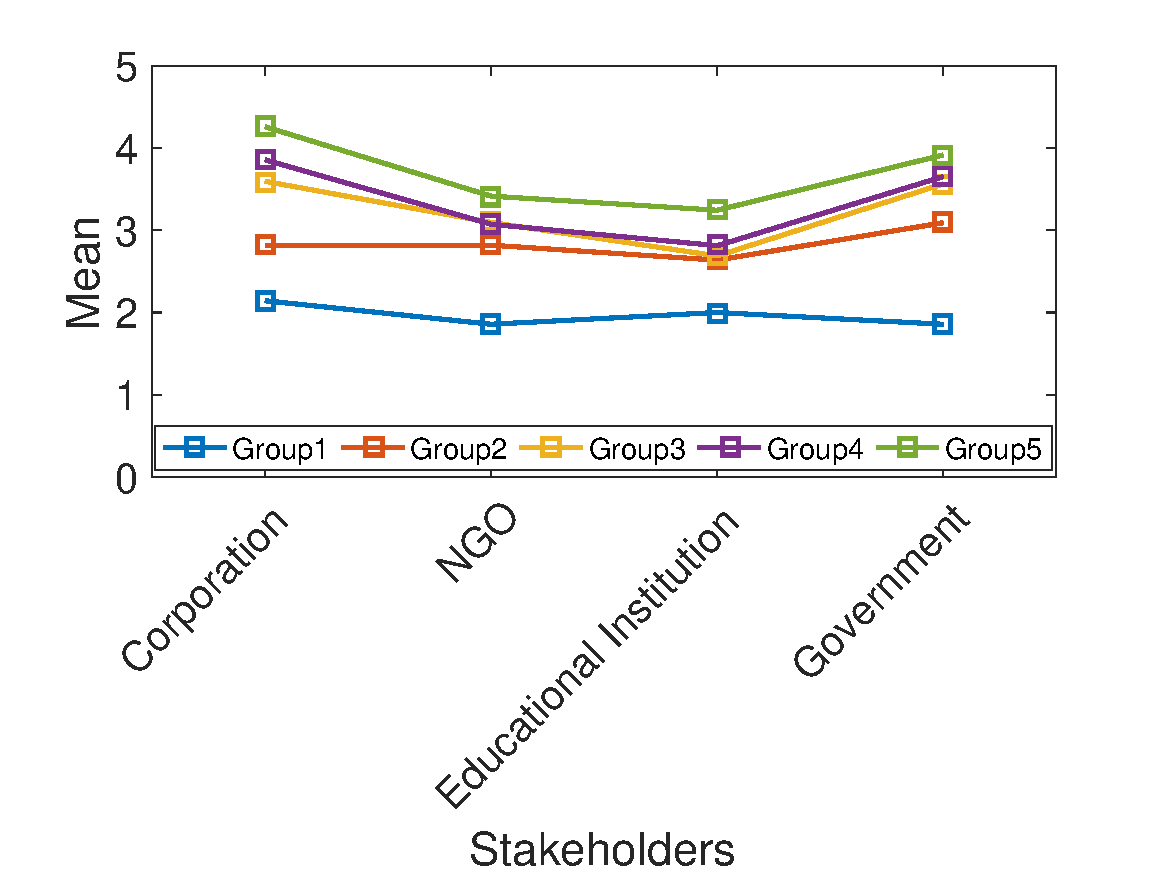
\includegraphics[width=0.55\linewidth]{./images/stakeholders_group_meanQ12}}
\subtop[Variance of each Group for each Stakeholder\label{fig:st2}]{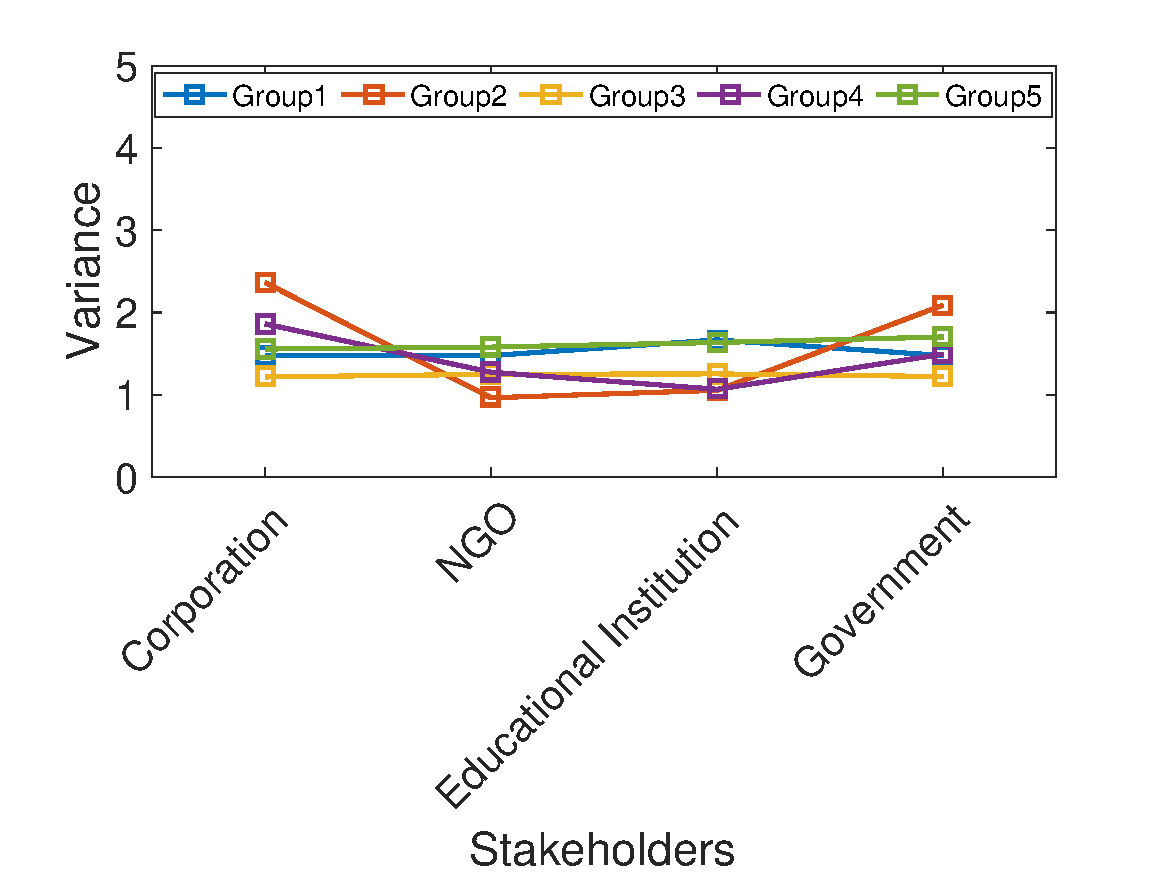
\includegraphics[width=0.55\linewidth]{./images/stakeholders_group_varianceQ12}}
\caption{Table Schemas}
\label{fig:st3}
\end{figure}

In this section, we try to see if the intrusion level perception by people of Stakeholders in general and the intrusion of the individual stakeholders are related. We try to examine significant differences between groups formed by using question 12's responses on the perception of
each stakeholder, and since there are 5 different responses this give five independent groups. The groups 1 to 5 have 7, 11, 32, 69 and 70 people in each respectively. More detailed information about the employment, education, gender and age distribution in the groups is given in tables \ref{tab:emp_stak}, \ref{tab:edu_stak}, \ref{tab:gender_stak} and \ref{tab:year_stak}.

The mean and variances of each group formed is depicted in figures \ref{fig:ss1} and \ref{fig:ss2}.
To start with we examine all the groups simultaneously for all the stakeholder's, we perform the Kruskal-Wallis H test since the data is discrete and not normally distributed. The null hypothesis is that the groups rate the intrusion of a particular stakeholder in a similar way. The alternative hypothesis is that the groups rate the intrusion of a particular stakeholder in a significantly different way.

The resulting p-values of this test is displayed in table \ref{kw_stak}. As it can be seen, the test pronounces that all the groups are significantly different at an alpha with 0.05. 

\begin{table}[h!]
  \centering
  \caption{Employment Classification of Groups}
  \label{tab:emp_stak}
  \begin{tabular}{cccccc}
    \toprule
     Occupation&1&2&3&4&5\\
    \midrule
Employed full time	&3.92\%	&4.90\%	&16.67\%	&33.33\%	&41.18\%\\
Employed part time	&16.67\%	&16.67\%	&8.33\%	&50.00\%	&8.33\%\\
Unemployed, looking for work	&8.33\%	&8.33\%	&16.67\%	&16.67\%	&50.00\%\\
Unemployed, not looking for work	&0.00\%	&0.00\%	&0.00\%	&33.33\%	&66.67\%\\
Retired	&0.00\%	&0.00\%	&0.00\%	&100.00\%&	0.00\%\\
Student	&4.82\%	&7.23\%	&15.66\%	&37.35\%	&34.94\%\\
Disabled	&0.00\%	&0.00\%	&0.00\%	&0.00\%	&0.00\%\\
    \bottomrule
  \end{tabular}
\end{table}



\begin{table}[h!]
  \centering
  \caption{Gender Classification of Groups}
  \label{tab:gender_stak}
  \begin{tabular}{cccccc}
    \toprule
     Gender&1&2&3&4&5 \\
     \midrule
Female&5.56\%&6.94\%&23.61\%&36.11\%&27.78\% \\
Male&3.97\%&6.35\%&11.90\%&35.71\%&42.06\%\\
    \bottomrule
  \end{tabular}
\end{table}



\begin{table}[h!]
  \centering
  \caption{Average Birth Year of Groups}
  \label{tab:year_stak}
  \begin{tabular}{ccccc}
    \toprule
     1&2&3&4&5\\
    \midrule
	1986& 1989& 1984& 1985& 1984\\
    \bottomrule
  \end{tabular}
\end{table}


\begin{table}[h!]
  \centering
  \caption{Education Classification of Groups}
  \label{tab:edu_stak}
  \begin{tabular}{cccccc}
    \toprule
     Education&1&2&3&4&5\\
    \midrule
    
Less than high school	&20.00\%	&20.00\%	&0.00\%	&60.00\%	&0.00\%\\
High school	& 15.79\%&	5.26\%	&21.05\%	&31.58\%	&26.32\%\\
Some college	 & 0.00\%&	10.00\%	&20.00\%	&40.00\%&	30.00\%\\
Bachelors degree 	&1.75\%	&12.28\%&	15.79\%	&35.09\%	&35.09\%\\
Masters degree	&5.06\%	&1.27\%	&13.92\%	&37.97\%	&41.77\%\\
PhD degree	&0.00\%	&7.14\%	&21.43\%	&28.57\%	&42.86\%\\
    \bottomrule
  \end{tabular}
\end{table}


\begin{table}[h!]
  \centering
  \caption{Kuskal-Wallis Test}
  \label{tab:kw_stak}
  \begin{tabular}{cc}
    \toprule
     Stakeholder & p-value \\
    \midrule
    Corporation & 2.1432e-05 \\
    Non-Governmental Organization & 0.0221\\
    Educational Institution & 0.0396\\
    Government & 0.0024\\ 
    \bottomrule
  \end{tabular}
\end{table}

This prompts us to take a closer look at which of the groups are significantly different from each other for each stakeholder. For this we continue the experiment with Dunn's Test with p-values adjusted by the Bonferroni Method. The results from the test is shown in table \ref{tab:dunn_stak}.

\begin{table}[h!]
  \centering
  \caption{Dunn's Test 1}
  \label{tab:dunn_stak}
  \begin{tabular}{ccccccc}
    \toprule
     Groups & Corporation & Non-Governmental Organization & Educational Institution & Government \\
    \midrule
    (1,2) & 0.9839 & 0.8042 & 0.9565 & 0.6615 \\
    (1,3) & 0.3282 & 0.2351 & 0.8540 & 0.0986 \\
    (1,4) & 0.0240 & 0.1962 & 0.6867 & 0.0289 \\
    (1,5) & 0.0012 & 0.0243 & 0.1254 & 0.0028 \\
    (2,3) & 0.9467 & 0.9992 & 1.0000 & 0.9958 \\
    (2,4) & 0.2047 & 0.9991 & 1.0000 & 0.9252  \\
    (2,5) & 0.0110 & 0.7192 & 0.8415 & 0.3670  \\
    (3,4) & 0.6893 & 1.0000 & 1.0000 & 0.9999 \\
    (3,5) & 0.0197 & 0.8906 & 0.4112 & 0.5794  \\
    (4,5) & 0.4640 & 0.6027 & 0.3427 & 0.7378 \\
    \bottomrule
  \end{tabular}
\end{table}  

\begin{figure}[htp]
\subtop[Mean of each Group for each Stakeholder\label{fig:st1}]{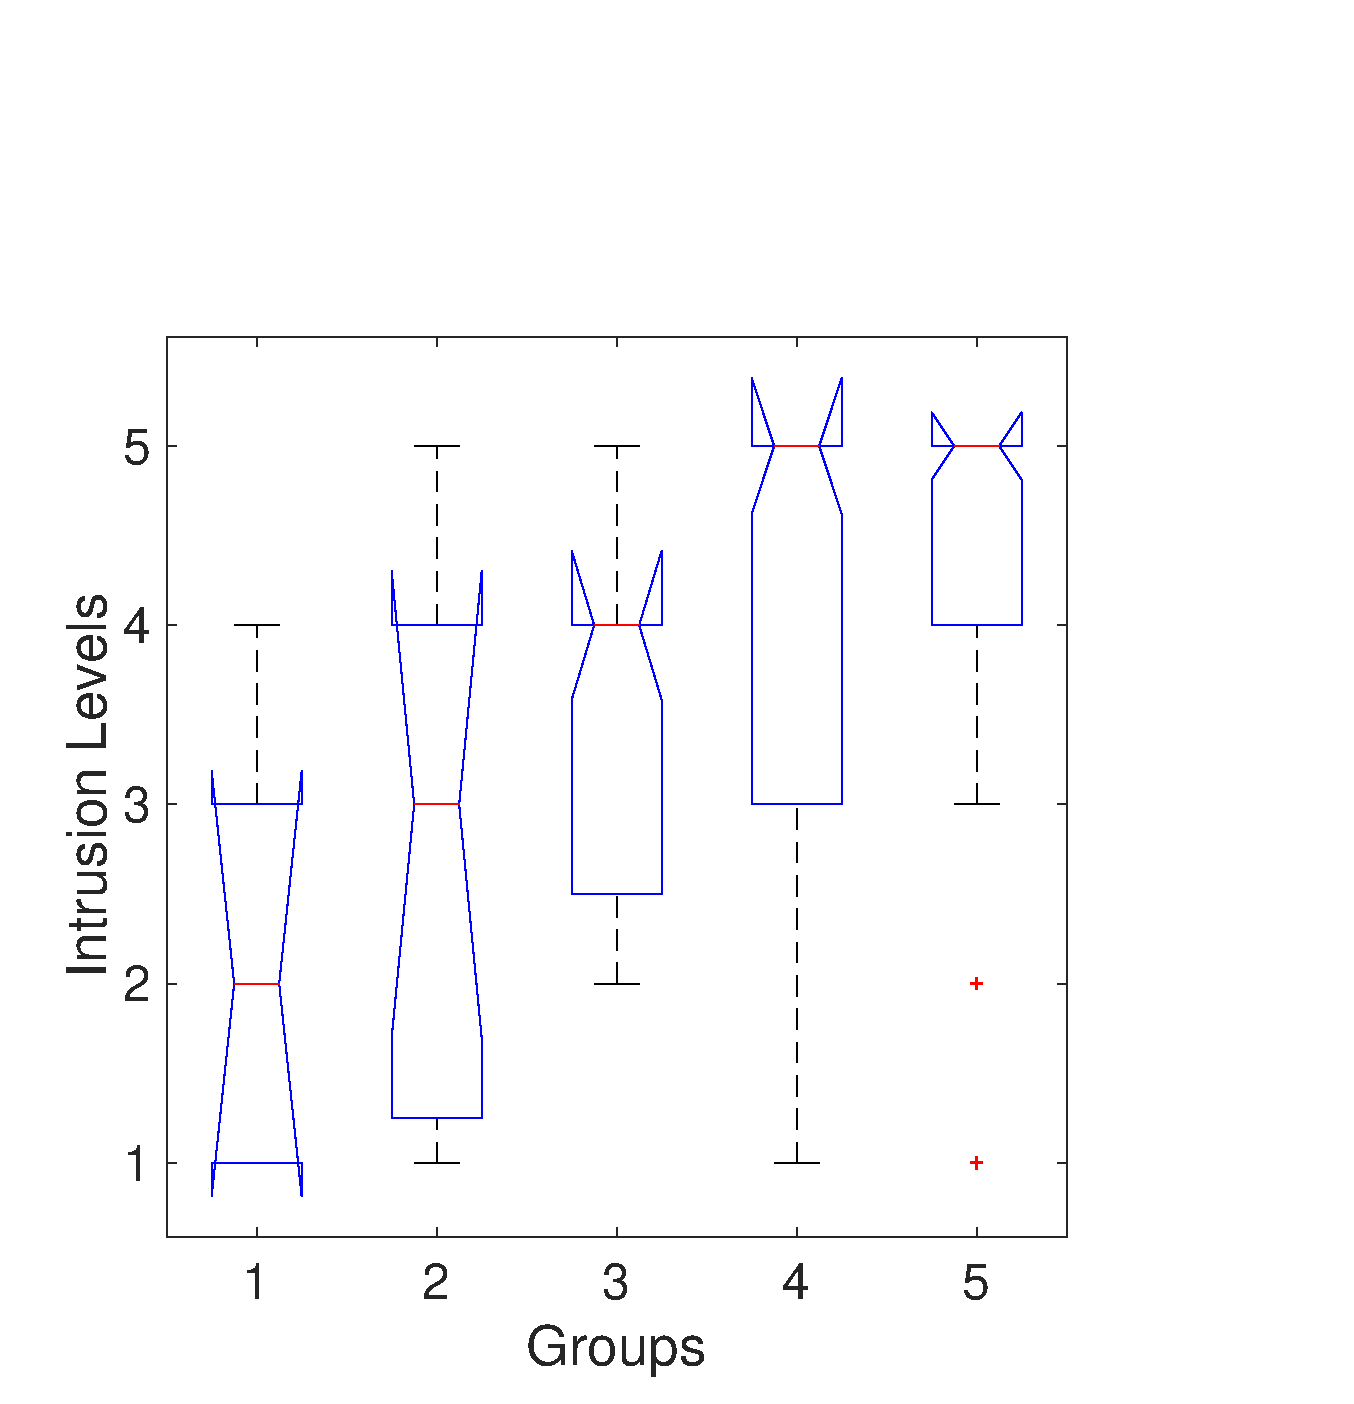
\includegraphics[width=0.4\linewidth]{./images/corp_box}}\hspace{1em}
\subtop[Variance of each Group for each Stakeholder\label{fig:st2}]{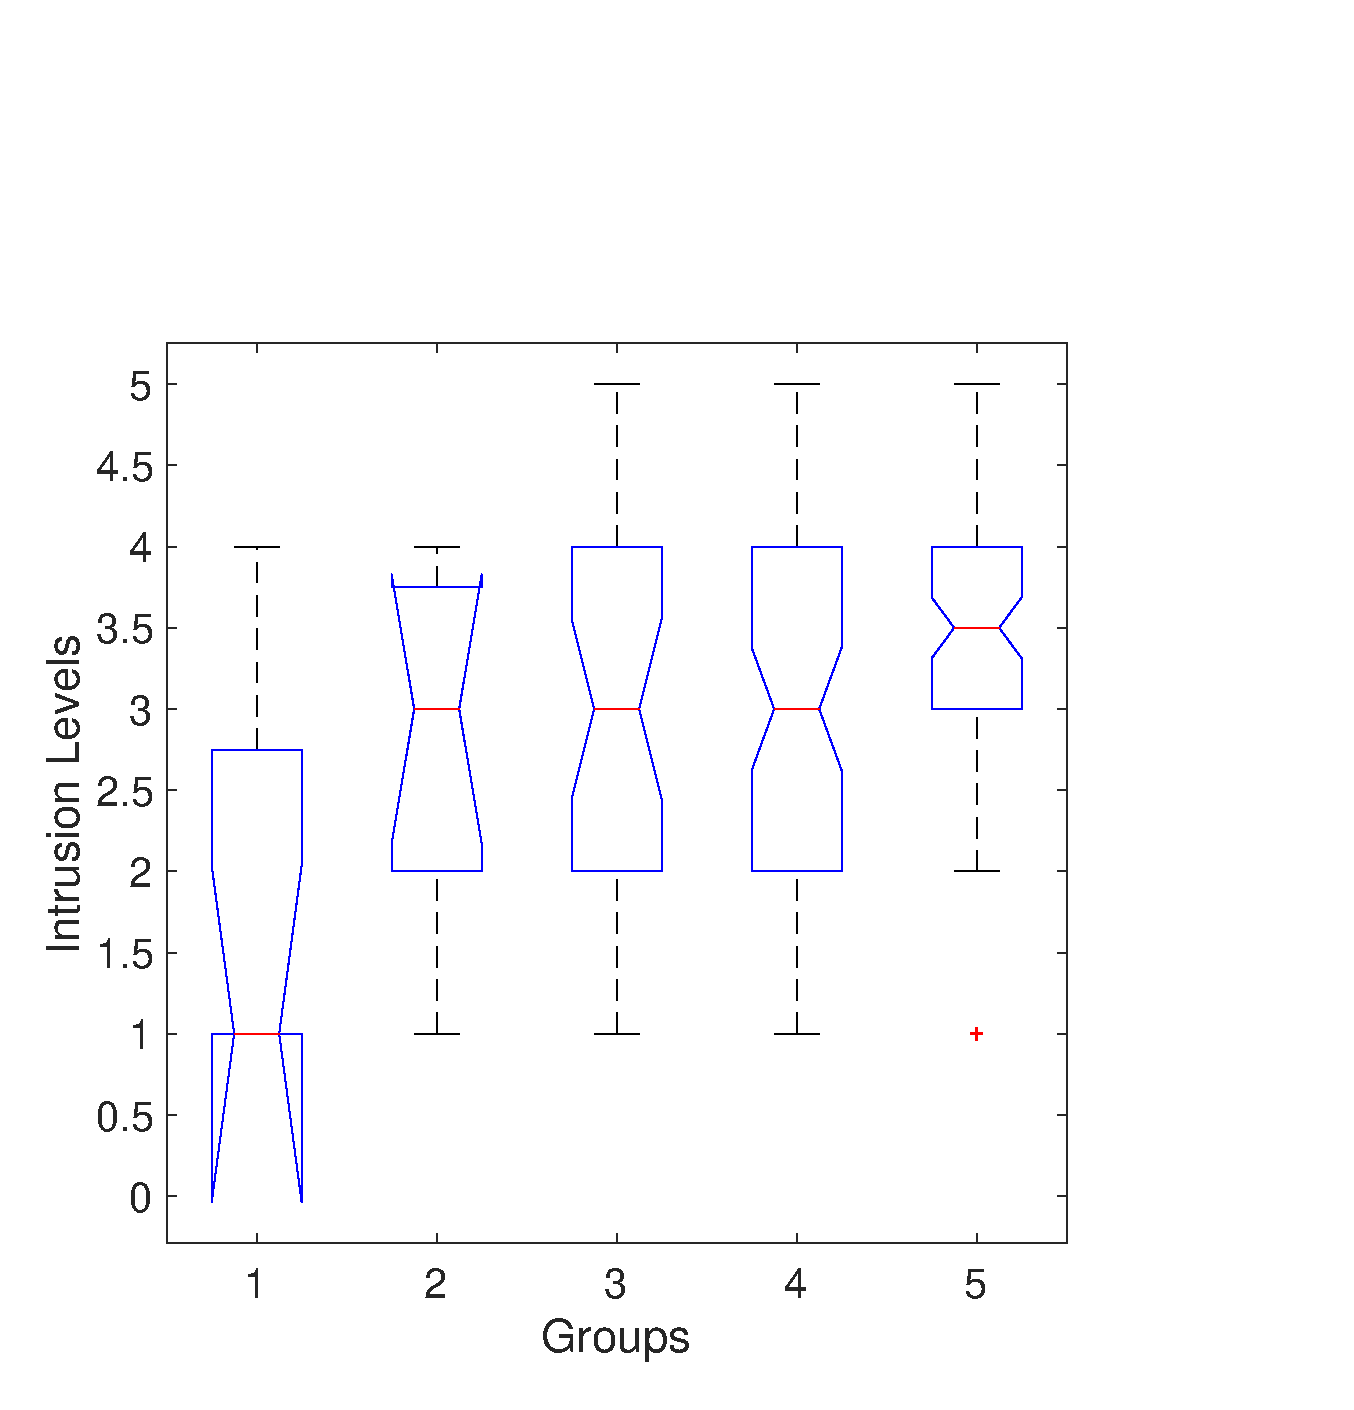
\includegraphics[width=0.4\linewidth]{./images/ngo_box}} \newline
\subtop[Variance of each Group for each Stakeholder\label{fig:st5}]{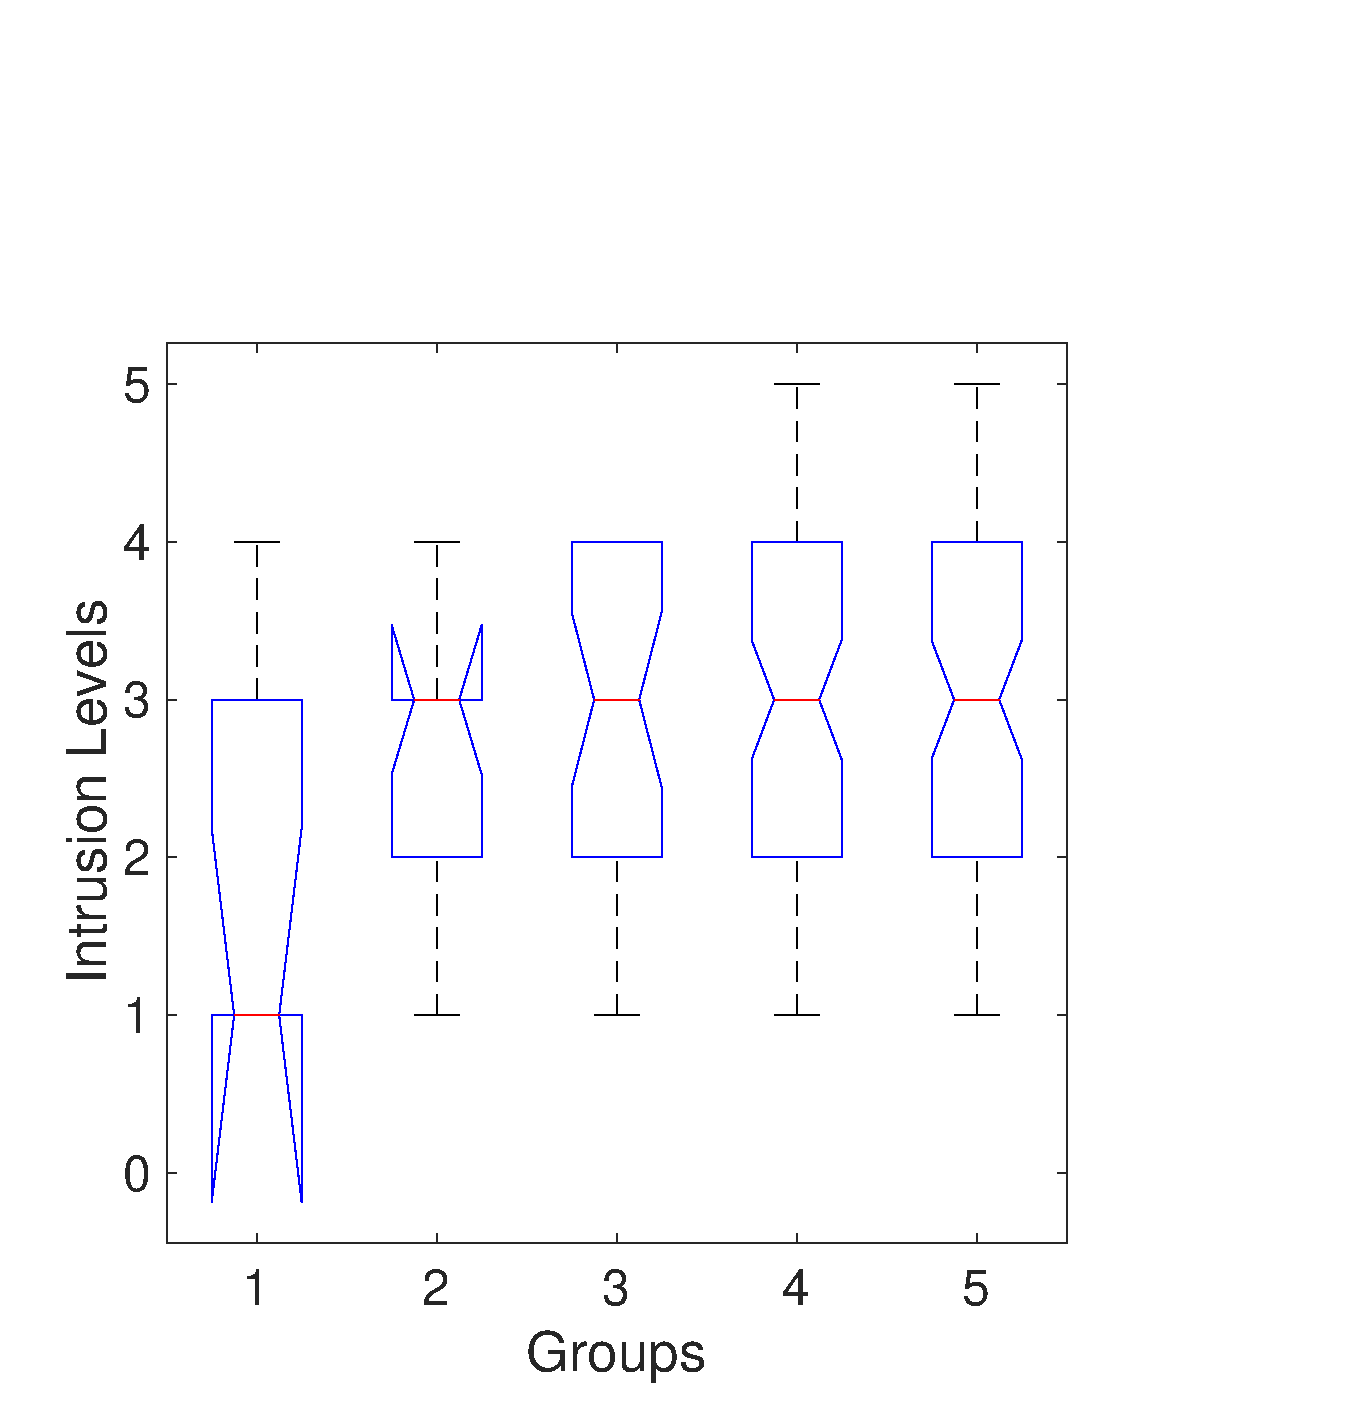
\includegraphics[width=0.4\linewidth]{./images/edu_box}}\hspace{1em}
\subtop[Variance of each Group for each Stakeholder\label{fig:st2}]{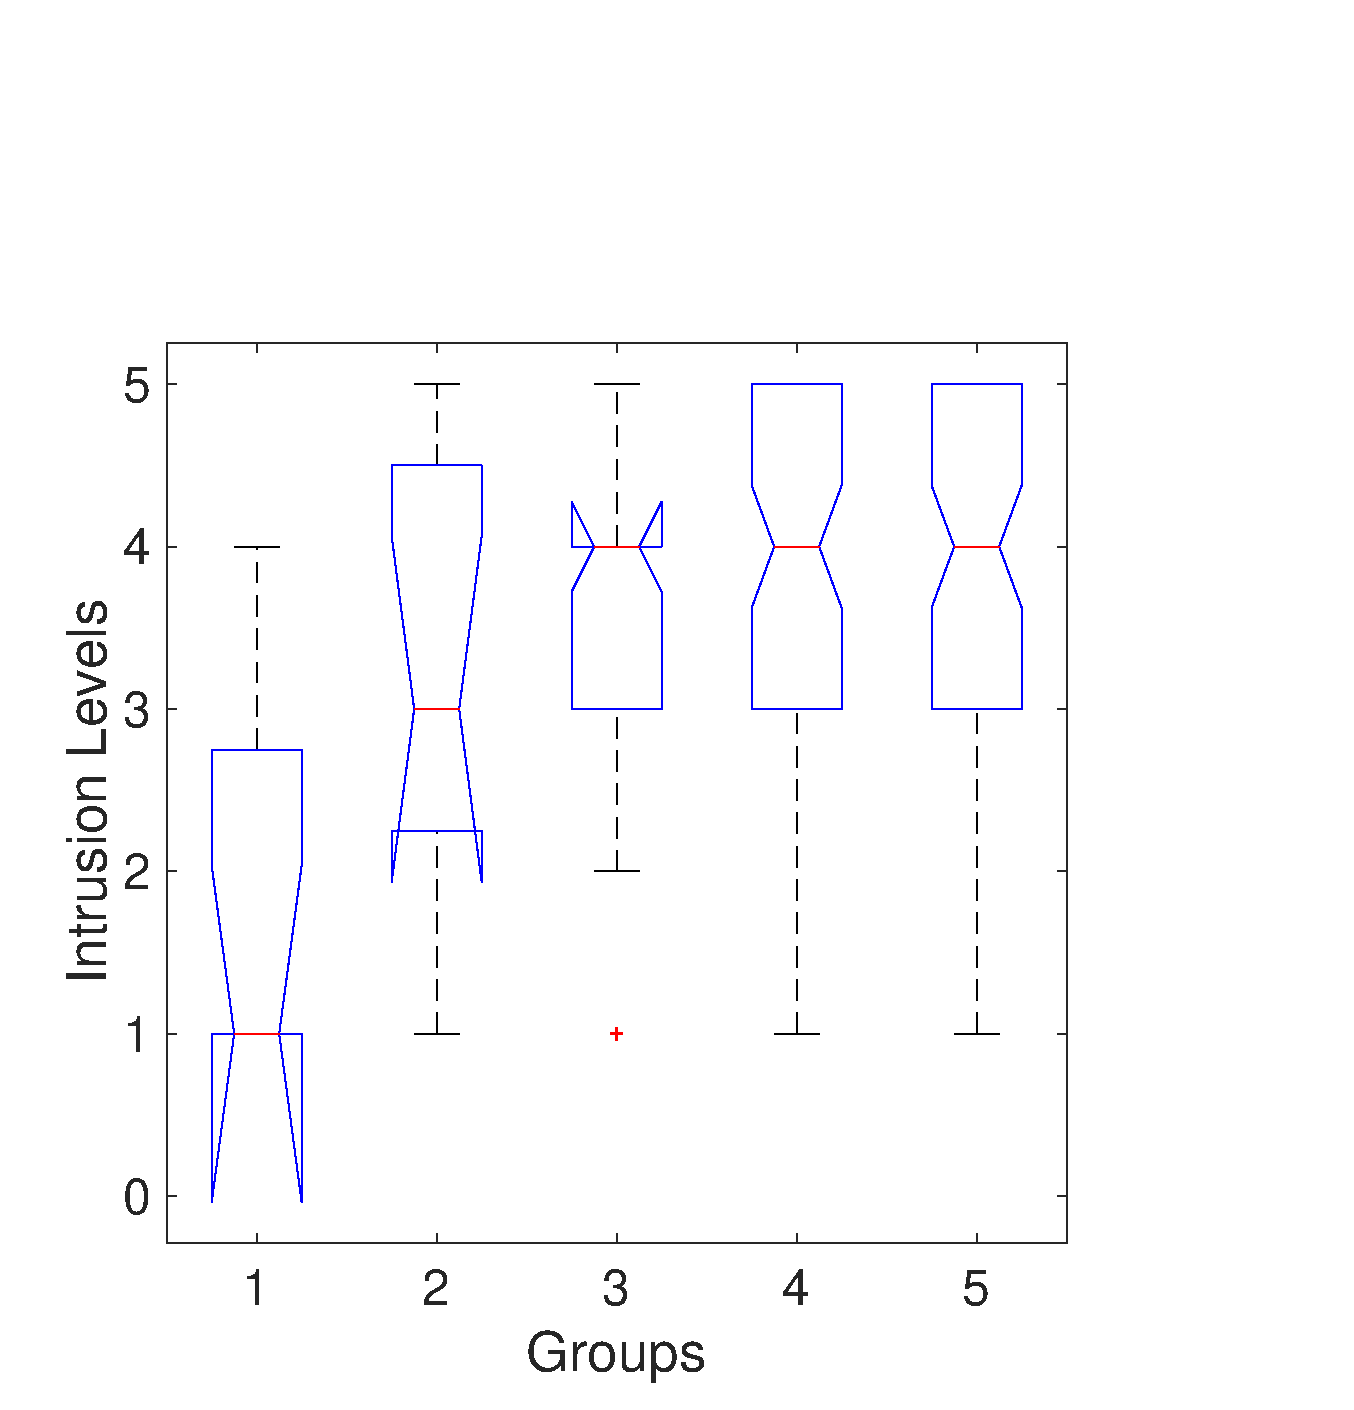
\includegraphics[width=0.4\linewidth]{./images/gov_box}} 
\caption{Table Schemas}
\label{fig:st3}
\end{figure}

The test was done for all stakeholders since the Kruskal-Wallis test denoted that all groups differ significantly for all stakeholders. Looking at the stakeholder corporation, we see that groups (1,4), (1,5) and (2,5). This goes to show that groups with larger difference in their outlook to stakeholders as a whole view corporations in a significantly different way.

For the Non-Governmental Organization, only the groups (1,5) differ significantly. This goes to show that groups that do not find stakeholders intrusive and groups that find stakeholders very intrusive rate the intrusion of Non-Governmental Organization in significantly different ways.

For Educational Institutions, none of pairwise comparisons have p-values below 0.05. This goes to show that the intrusion of Educational Institutions by all groups does not differ significantly.

Lastly, for the stakeholder Government, the groups (1,4) and (1,5) differ significantly. This goes to show that groups that view the intrusion of stakeholders with a larger difference view Government in a significantly different way.

The trend observed above is that there is a significant difference in the outlook of individual stakeholders between groups with larger differences
in their outlook to stakeholders as a whole, with the exception of Educational Institution where the alternative hypothesis was rejected.


\subsubsection{Perception of Individual Contexts Grouped on the Intrusion of Contexts in General}

\begin{figure}[htp]
\subtop[Mean of each Group for each Context\label{fig:co1}]{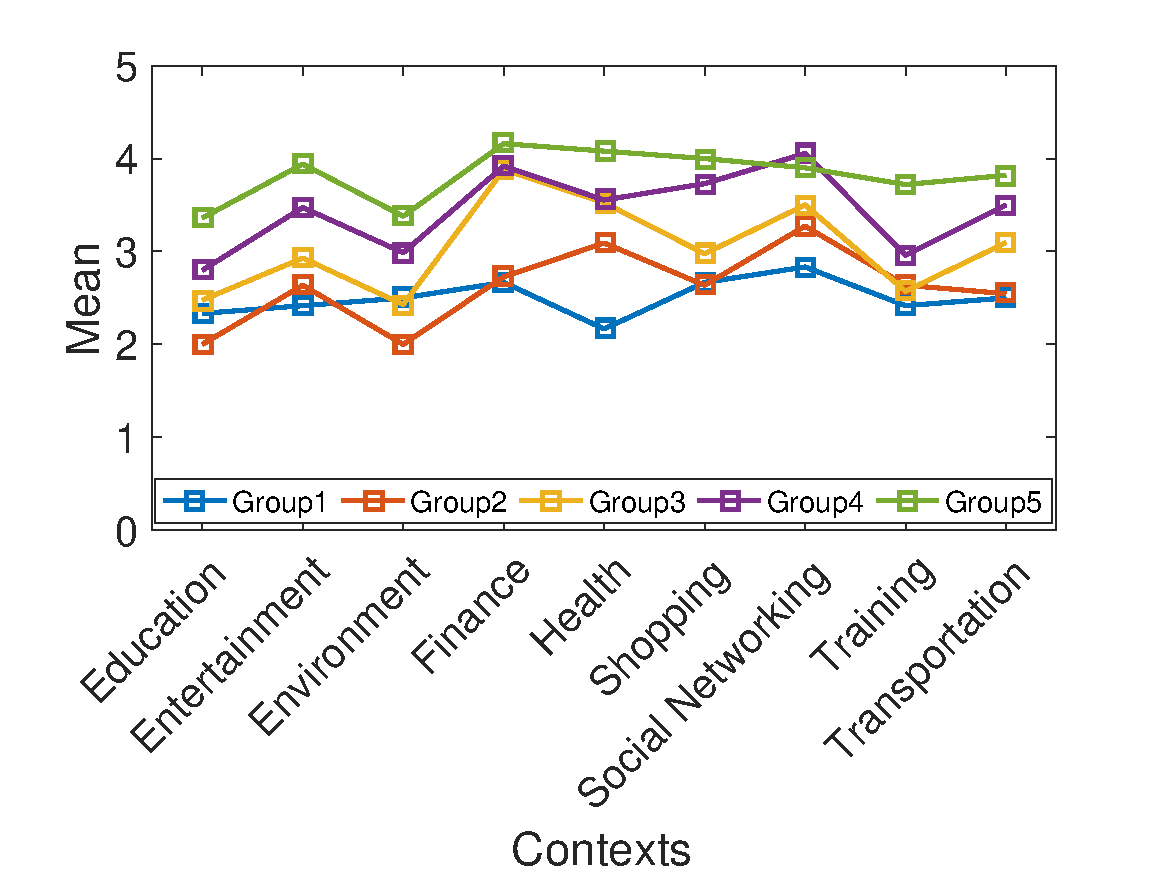
\includegraphics[width=0.55\linewidth]{./images/contexts_group_meanQ14}}
\subtop[Variance of each Group for each Context\label{fig:co2}]{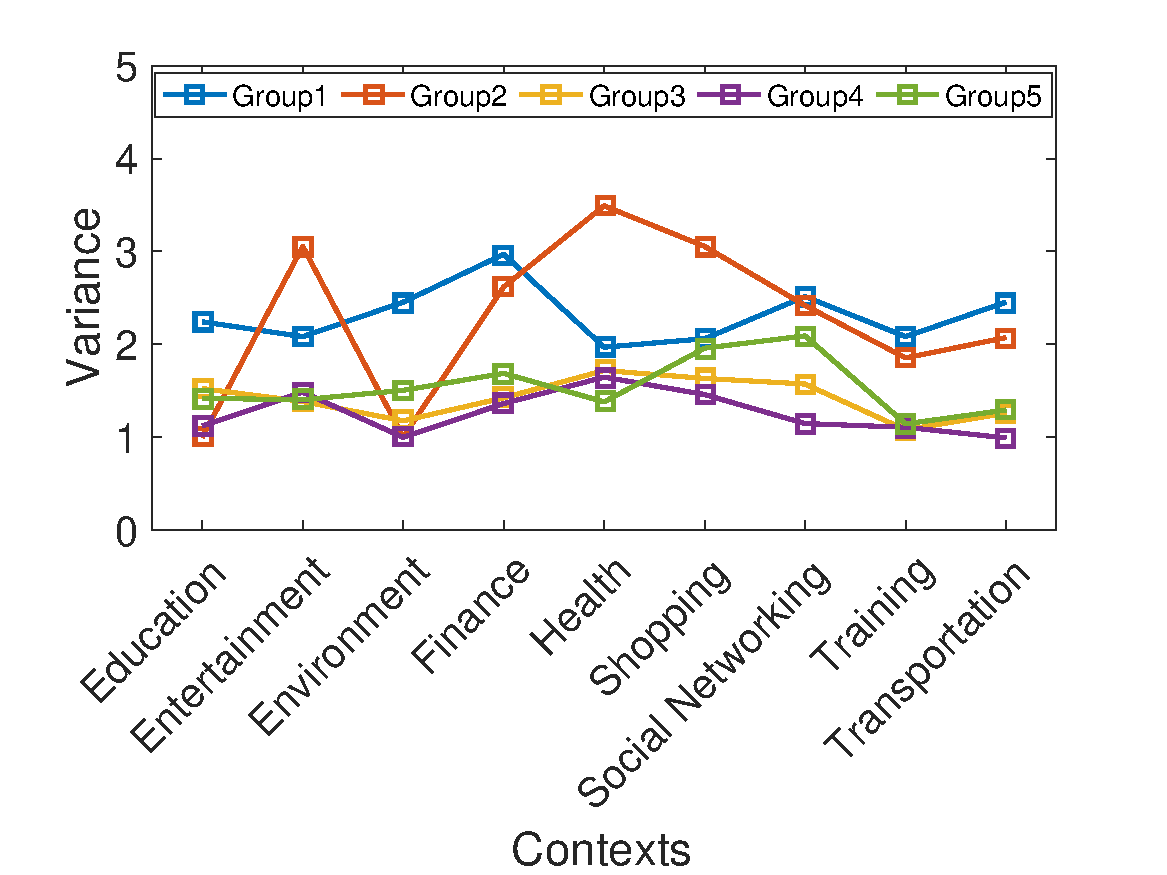
\includegraphics[width=0.55\linewidth]{./images/contexts_group_varianceQ14}}
\caption{Table Schemas}
\label{fig:co3}
\end{figure}

In this section, we examine the examine the relationship between the intrusion of Contexts in General and the individual contexts in question 13.
To do this, like the above sections we partition the data into groups based on the answers given questions 14, which asks the user the perception of intrusion of Contexts in general. There are five groups in total. Group one to five have each 12, 11, 42, 74 and 50 people respectively. Additional
information about the groups on enployment, education , gender and year of birth is given in tables \ref{tab:emp_c}, \ref{tab:edu_c}, \ref{tab:gender_c} and \ref{tab:year_c}. 

Like in the previous cases, since the data is discrete and not normal, we use the Kruskal-Wallis test to compare the groups perceptions on various contexts. The alpha value is considered to be 0.05. The results are presented in table \ref{tab:kw_c}. As it can be seen, the test says that there is a significant difference between the groups for all sensors.

\begin{table}[h!]
  \centering
  \caption{Employment Classification of Groups}
  \label{tab:emp_c}
  \begin{tabular}{cccccc}
    \toprule
     Occupation&1&2&3&4&5\\
    \midrule
Employed full time	&4.90\%	&3.92\%	&23.53\%	&36.27\%	&31.37\%\\
Employed part time	&16.67\%	&8.33\%	&25.00\%	&25.00\%	&25.00\%\\
Unemployed, looking for work	&8.33\%	&16.67\%	&25.00\%	&25.00\%	&25.00\%\\
Unemployed, not looking for work	&0.00\%	&0.00\%	&0.00\%	&66.67\%	&33.33\%\\
Retired	&0.00\%	&0.00\%	&0.00\%	&100.00\% &	0.00\%\\
Student	&7.23\%	&6.02\%	&20.48\%	&44.58\%	&21.69\%\\
Disabled	&0.00\%	&0.00\%	&0.00\%	&0.00\%	&0.00\%\\
    \bottomrule
  \end{tabular}
\end{table}



\begin{table}[h!]
  \centering
  \caption{Gender Classification of Groups}
  \label{tab:gender_c}
  \begin{tabular}{cccccc}
    \toprule
     Gender&1&2&3&4&5 \\
    \midrule
Male&	7.14\%	&6.35\%	&23.02\%	&38.10\%	&25.40\% \\
Female	&5.56\%	&5.56\%	&19.44\%	&38.89\%	&30.56\% \\
    \bottomrule
  \end{tabular}
\end{table}



\begin{table}[h!]
  \centering
  \caption{Average Birth Year of Groups}
  \label{tab:year_c}
  \begin{tabular}{ccccc}
    \toprule
     1&2&3&4&5\\
    \midrule
	1986& 1986& 1986& 1985& 1983\\
    \bottomrule
  \end{tabular}
\end{table}


\begin{table}[h!]
  \centering
  \caption{Education Classification of Groups}
  \label{tab:edu_c}
  \begin{tabular}{cccccc}
    \toprule
     Education&1&2&3&4&5\\
    \midrule
    
Less than high school	&20.00\%	&0.00\%	&0.00\%	&80.00\%	&0.00\%\\
High school	&10.53\%	&10.53\%	&31.58\%	&36.84\%	&10.53\%\\
Some college	1&0.00\%	&0.00\%	&40.00\%	&30.00\%	&20.00\%\\
Bachelors degree	&7.02\%	&8.77\%	&24.56\%	&35.09\%	&24.56\%\\
Masters degree	&6.33\%	&3.80\%	&17.72\%	&40.51\%	&31.65\%\\
PhD degree	&0.00\%	&7.14\%	&17.86\%	&35.71\%	3&9.29\%\\
    \bottomrule
  \end{tabular}
\end{table}  


\begin{table}[h!]
  \centering
  \caption{Kuskal-Wallis Test}
  \label{tab:kw_c}
  \begin{tabular}{cc}
    \toprule
     Context & p-value \\
    \midrule
    Education &  6.4694e-04 \\
    Entertainment & 1.0660e-04\\
    Environment & 1.3079e-04\\
    Finance & 0.0021\\ 
    Health & 0.0011\\
    Shopping & 5.4227e-05\\ 
    Social Network &  0.0120\\
    Training & 1.2071e-05\\
    Transportation & 4.9043e-04\\ 
    \bottomrule
  \end{tabular}
\end{table} 


\begin{table}[h!]
  \centering
  \caption{Dunn's Test Part 1}
  \label{tab:dunn_c}
  \begin{tabular}{cccccccc}
    \toprule
     Groups & Education & Entertainment & Environment & Finance & Health  \\
    \midrule
    (1,2)&0.99796&0.99982&0.97055&1.0000&0.63908\\
(1,3)&1.0000&0.99174&1&0.32963&0.076147\\
(1,4)&0.94148&0.19262&0.86998&0.22077&0.042547\\
(1,5)&0.11471&0.0056283&0.21553&0.015364&0.00051115\\
(2,3)&0.9342&1&0.96665&0.31604&0.9999\\
(2,4)&0.32744&0.76121&0.083389&0.21508&0.99963\\
(2,5)&0.0082212&0.082023&0.0048936&0.016365&0.50246\\
(3,4)&0.83617&0.23034&0.10875&1.0000&1.0000\\
(3,5)&0.0064191&0.00086418&0.0012905&0.65747&0.32713\\
(4,5)&0.13825&0.28231&0.60016&0.57519&0.21258\\
    \bottomrule
  \end{tabular}
\end{table}

\begin{table}[h!]
  \centering
  \caption{Dunn's Test Part 2}
  \label{tab:dunn_c1}
  \begin{tabular}{ccccccc}
    \toprule
     Groups & Shopping & Social Network & Training & Transportation  \\
    \midrule
(1,2) &1.0000&0.99831&1.0000&1.0000\\
(1,3)&0.99992&0.94767&1.0000&0.9722\\
(1,4)&0.18309&0.089135&0.90197&0.23809\\
(1,5)&0.015842&0.10636&0.010906&0.016376\\
(2,3)&1.0000&1.0000&1&0.98253\\
(2,4)&0.39426&0.70552&0.99778&0.30509\\
(2,5)&0.052334&0.7272&0.068368&0.026144\\
(3,4)&0.038351&0.21259&0.58123&0.51397\\
(3,5)&0.00050454&0.29374&2.1697e-05&0.012924\\
(4,5)&0.69535&1.0000&0.0033189&0.55629\\
  \end{tabular}
\end{table} 

We not perform Dunn's Test as a post hoc test for all the contexts to observe the exact group pairs that might be significantly different. The results are presented in tables \ref{tab:dunn_c} and \ref{tab:dunn_c1}. For the context Education, the groups (2,5) and (3,5) are significantly different from each other. 
For the context Entertainment, further investigation shows that groups (1,5), (2,5) and (3,5) are significantly different in each others responses.
For the context Environment, groups (2,5) and (3,5) are significantly different from each other. For the context Finance, the groups (1,5), (3,5) and (4,5) are significantly different from each other. In the context health, except for groups (1,5) all the other groups are not significantly different from each other.
For the context Shopping, the groups (1,5), (3,4) and (3,5) are significantly different from each other. For the context Social Network, none of the groups are significantly different from each other. In the context Training, the groups (1,5),(3,5) and (4,5) are significantly different from each other.
Finally for the context Transportation, the groups (1,5), (2,5) and (3,5) are significantly different from each other.

This goes to show that groups that perceive contexts in a more different light tend to have different ways of viewing the individual contexts. We do observe that in some cases (2,5) are significantly different, but (1,5) is not. This can be easily attributed to the low number of responses
and the noise in the data.

\begin{figure}[htp]

\subtop[Mean of each Group for each Stakeholder\label{fig:st1}]{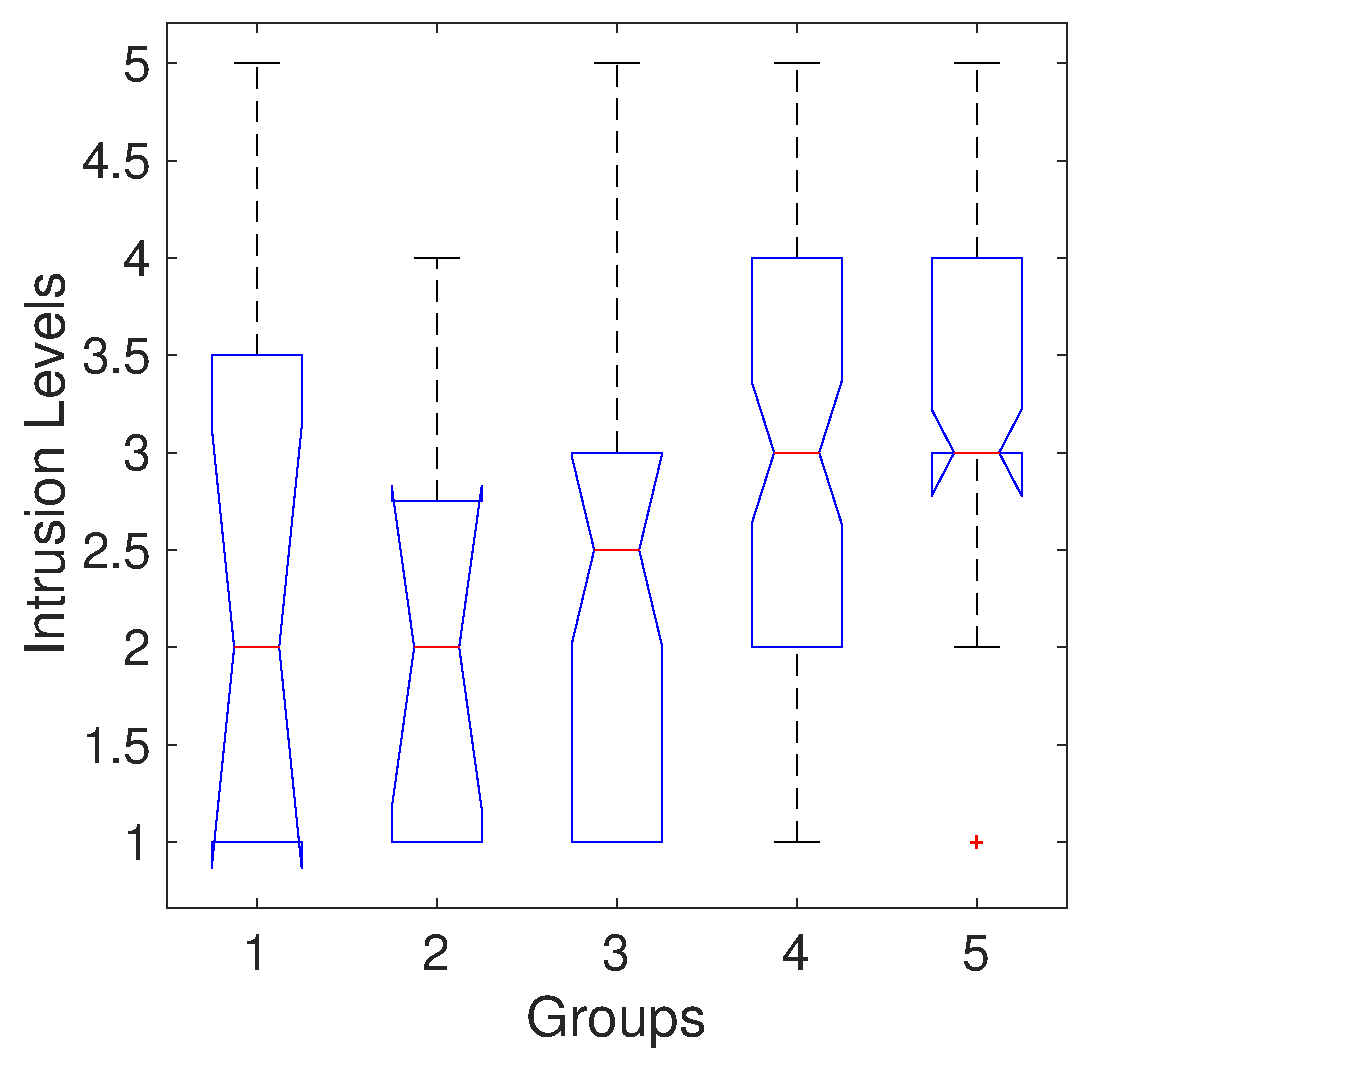
\includegraphics[width=0.4\linewidth]{./images/educ_box}}\hspace{1em}
\subtop[Variance of each Group for each Stakeholder\label{fig:st2}]{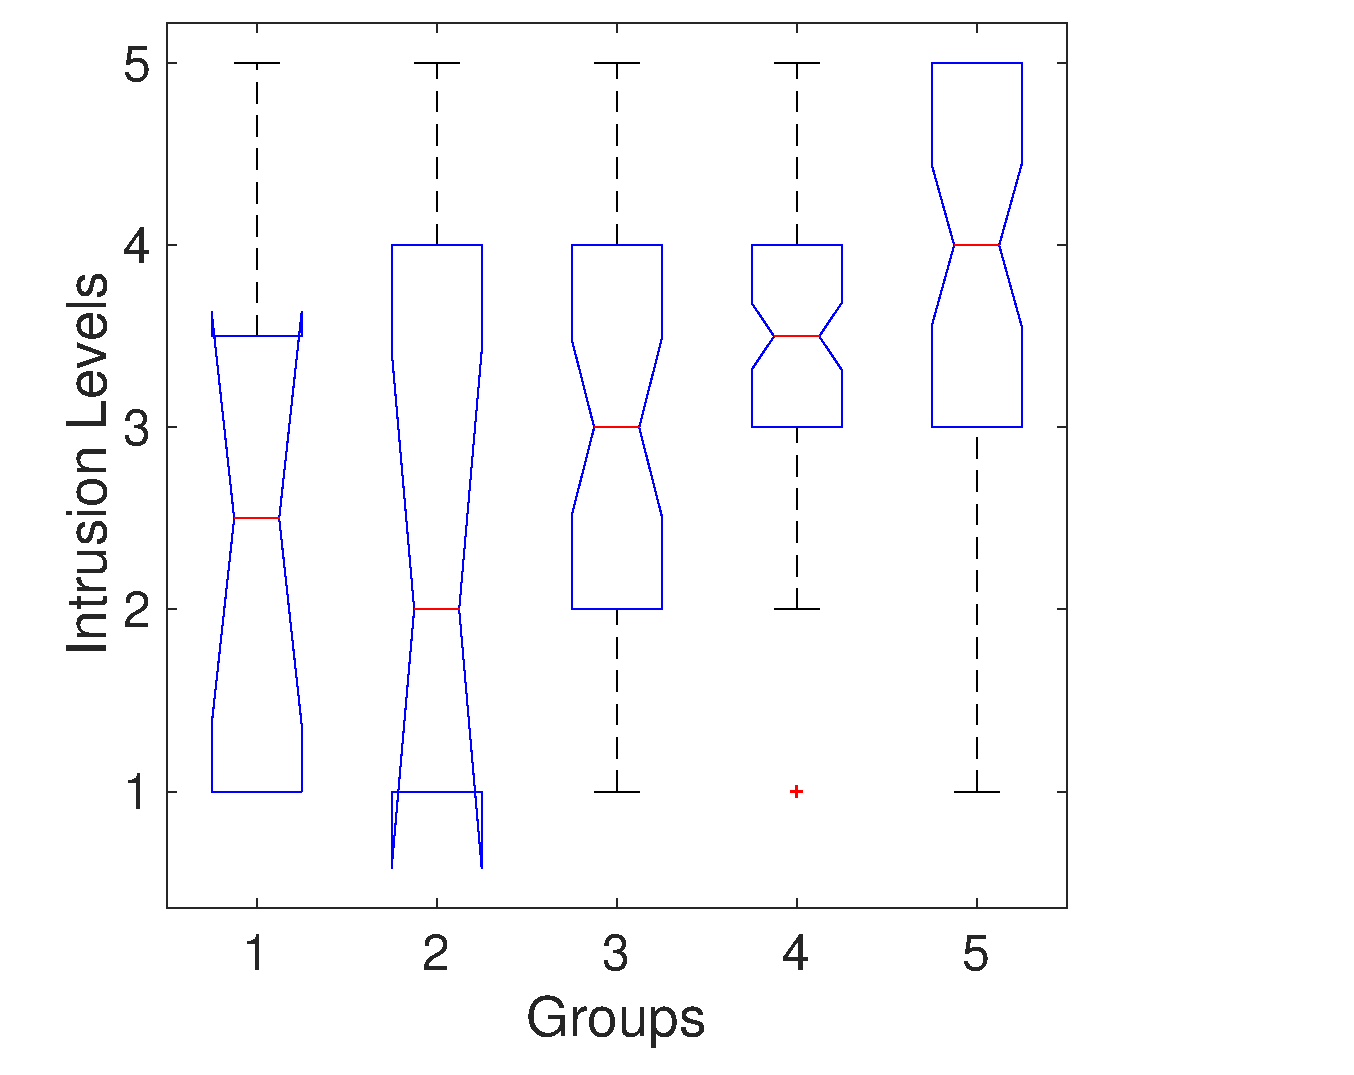
\includegraphics[width=0.4\linewidth]{./images/ent_box}} \newline
\subtop[Variance of each Group for each Stakeholder\label{fig:st5}]{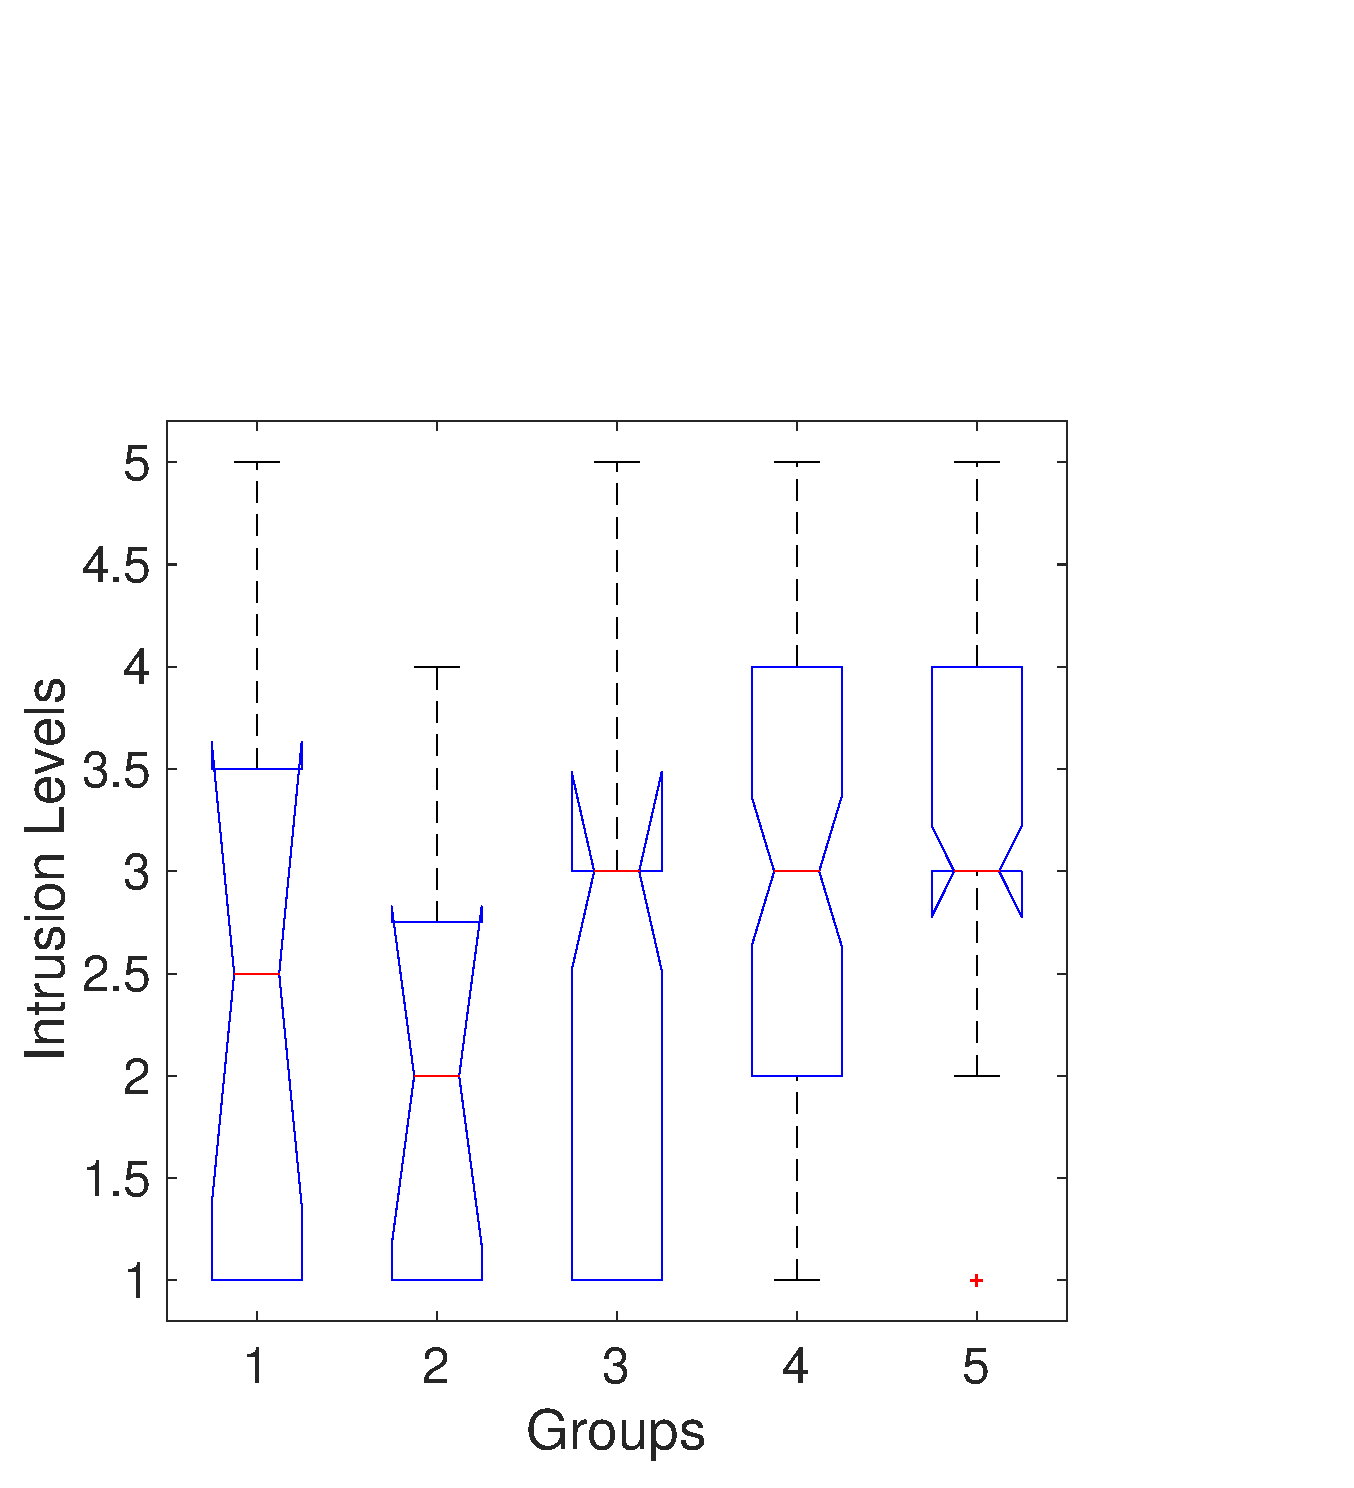
\includegraphics[width=0.4\linewidth]{./images/env_box}}\hspace{1em}
\subtop[Variance of each Group for each Stakeholder\label{fig:st2}]{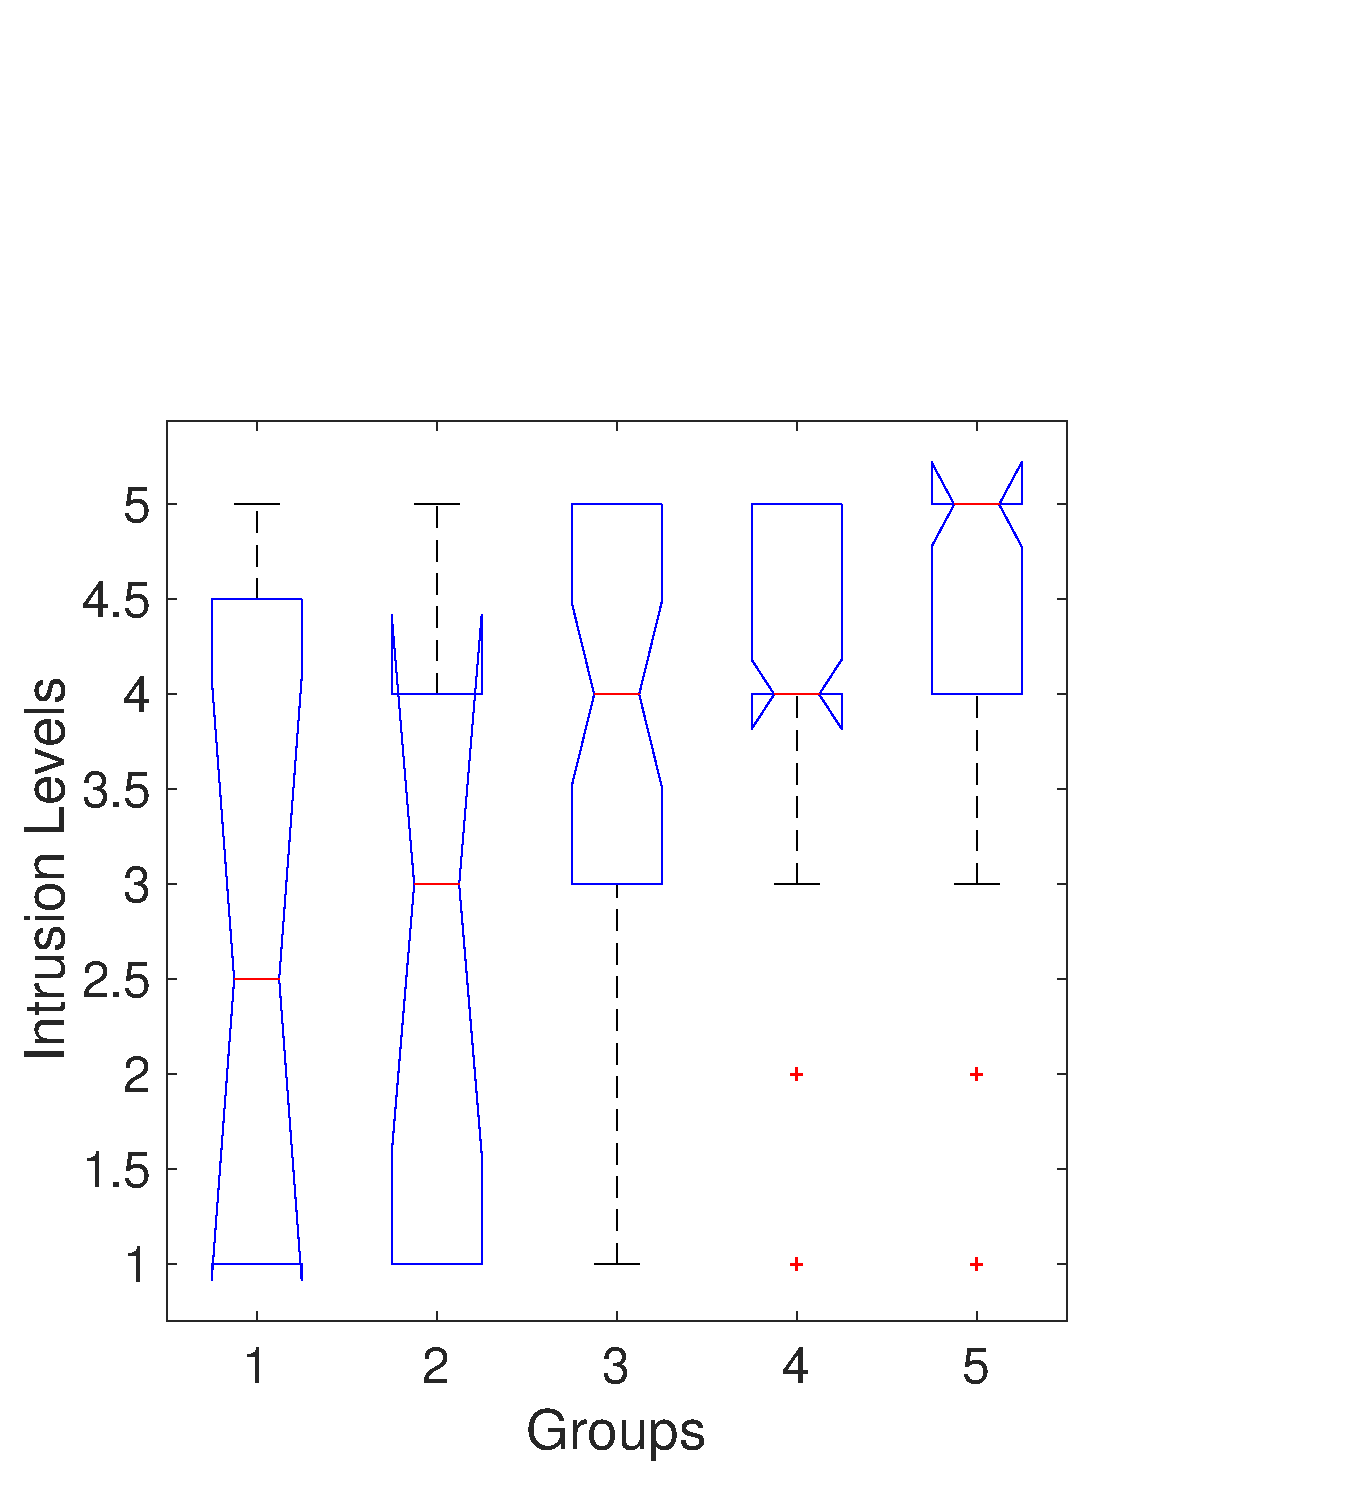
\includegraphics[width=0.4\linewidth]{./images/finance_box}} \newline
\subtop[Variance of each Group for each Stakeholder\label{fig:st5}]{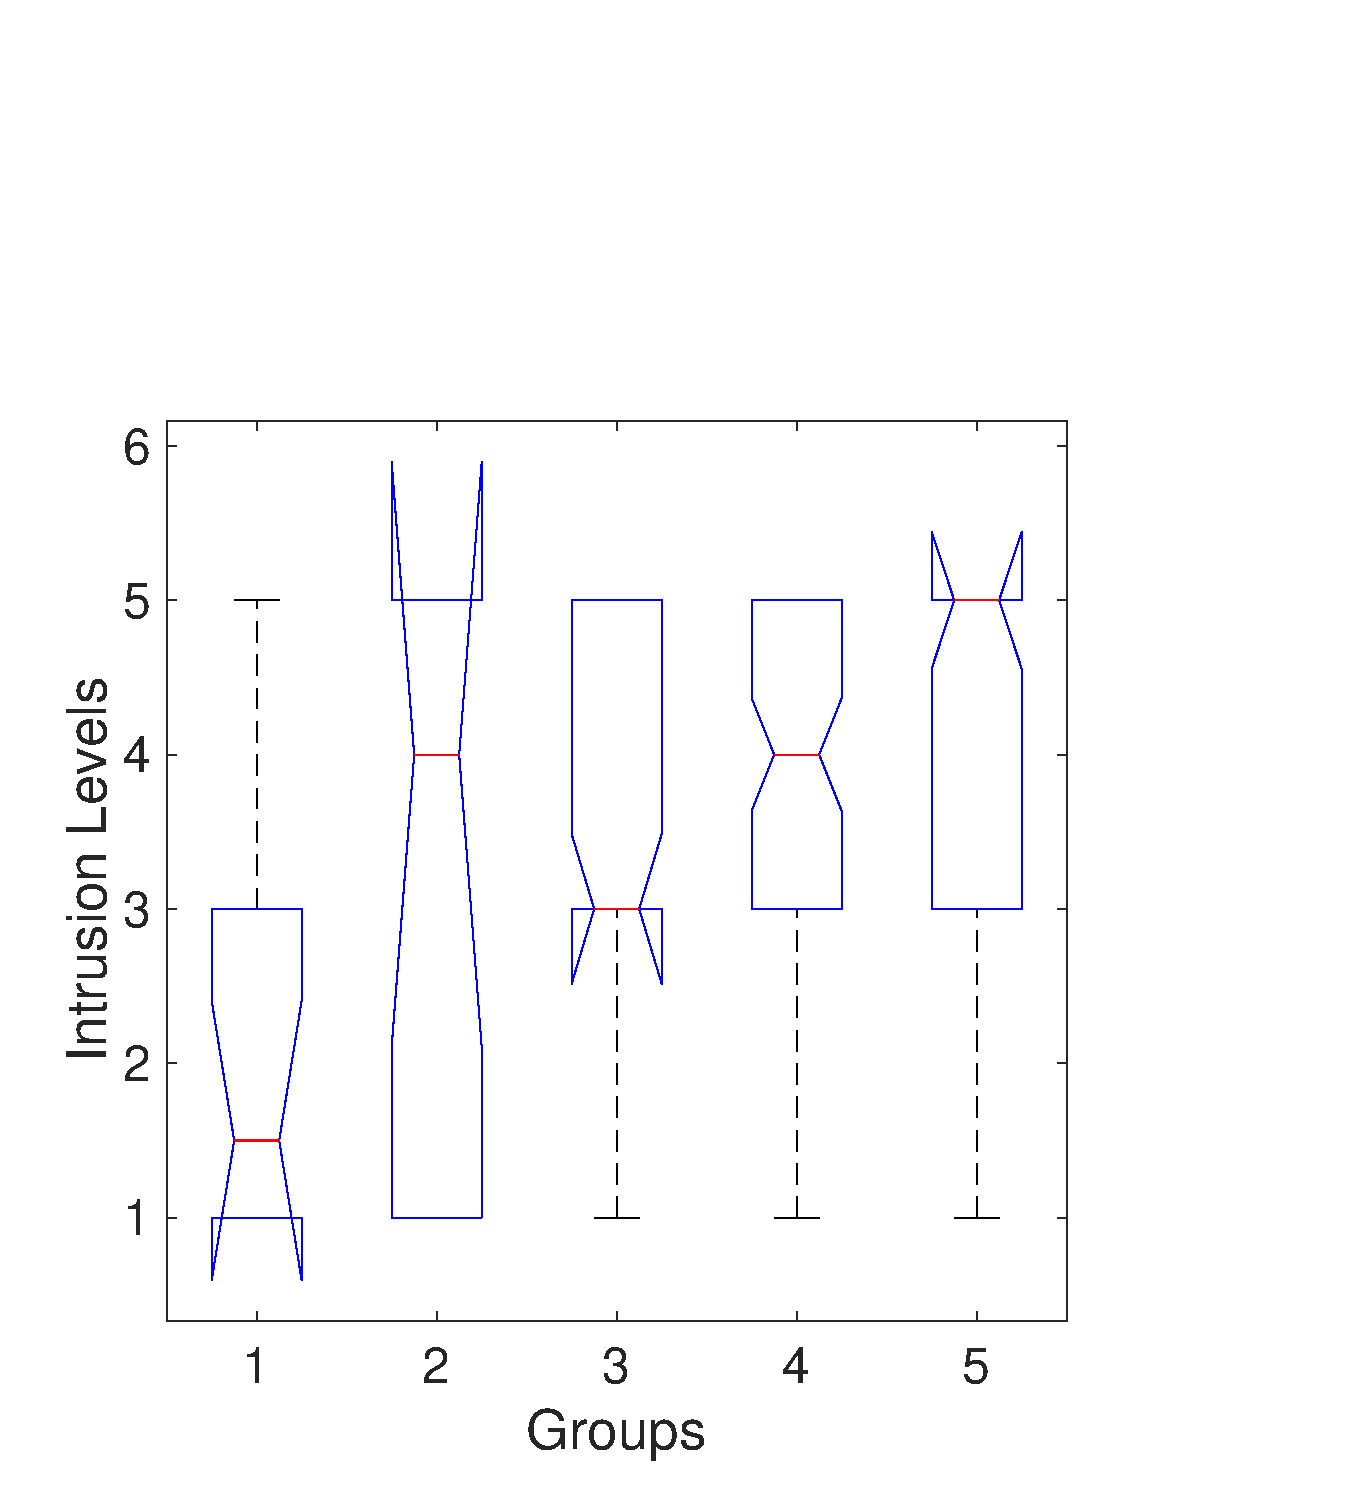
\includegraphics[width=0.4\linewidth]{./images/health_box}}\hspace{1em}
\subtop[Variance of each Group for each Stakeholder\label{fig:st2}]{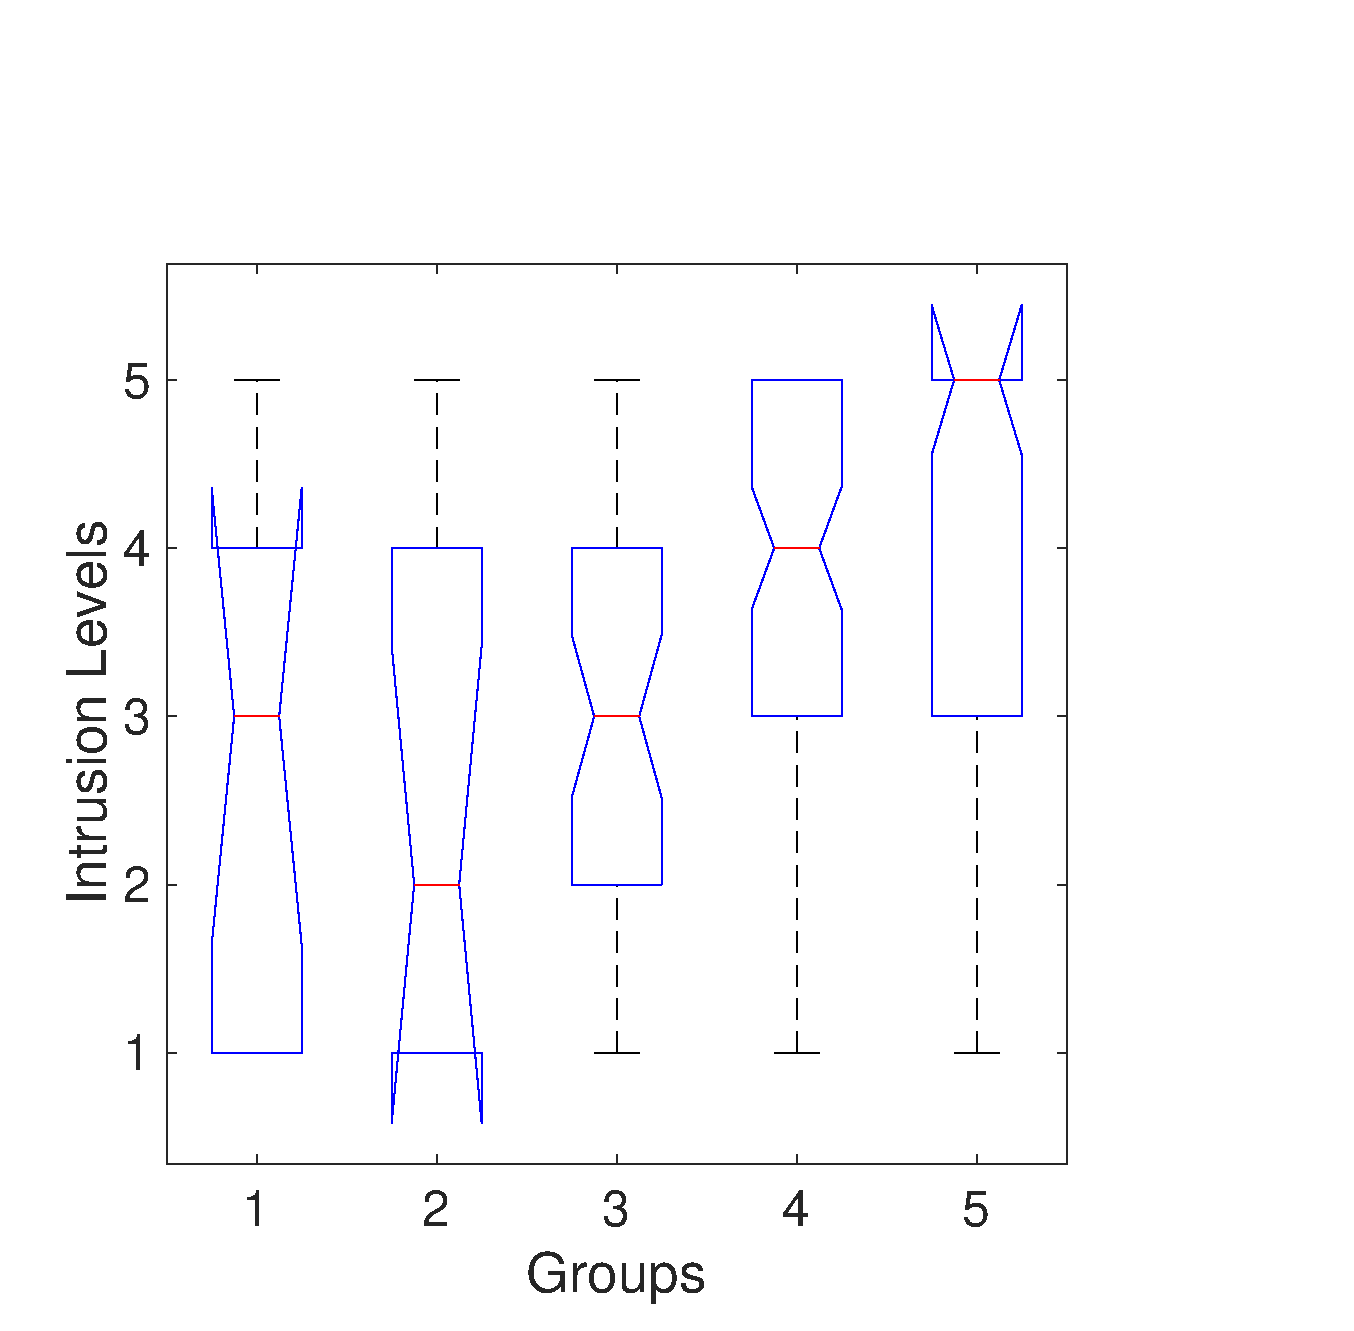
\includegraphics[width=0.4\linewidth]{./images/shopping_box}} 
\caption{Table Schemas}
\label{fig:st3}
\end{figure}

\begin{figure}[htp]
\subtop[Variance of each Group for each Stakeholder\label{fig:st5}]{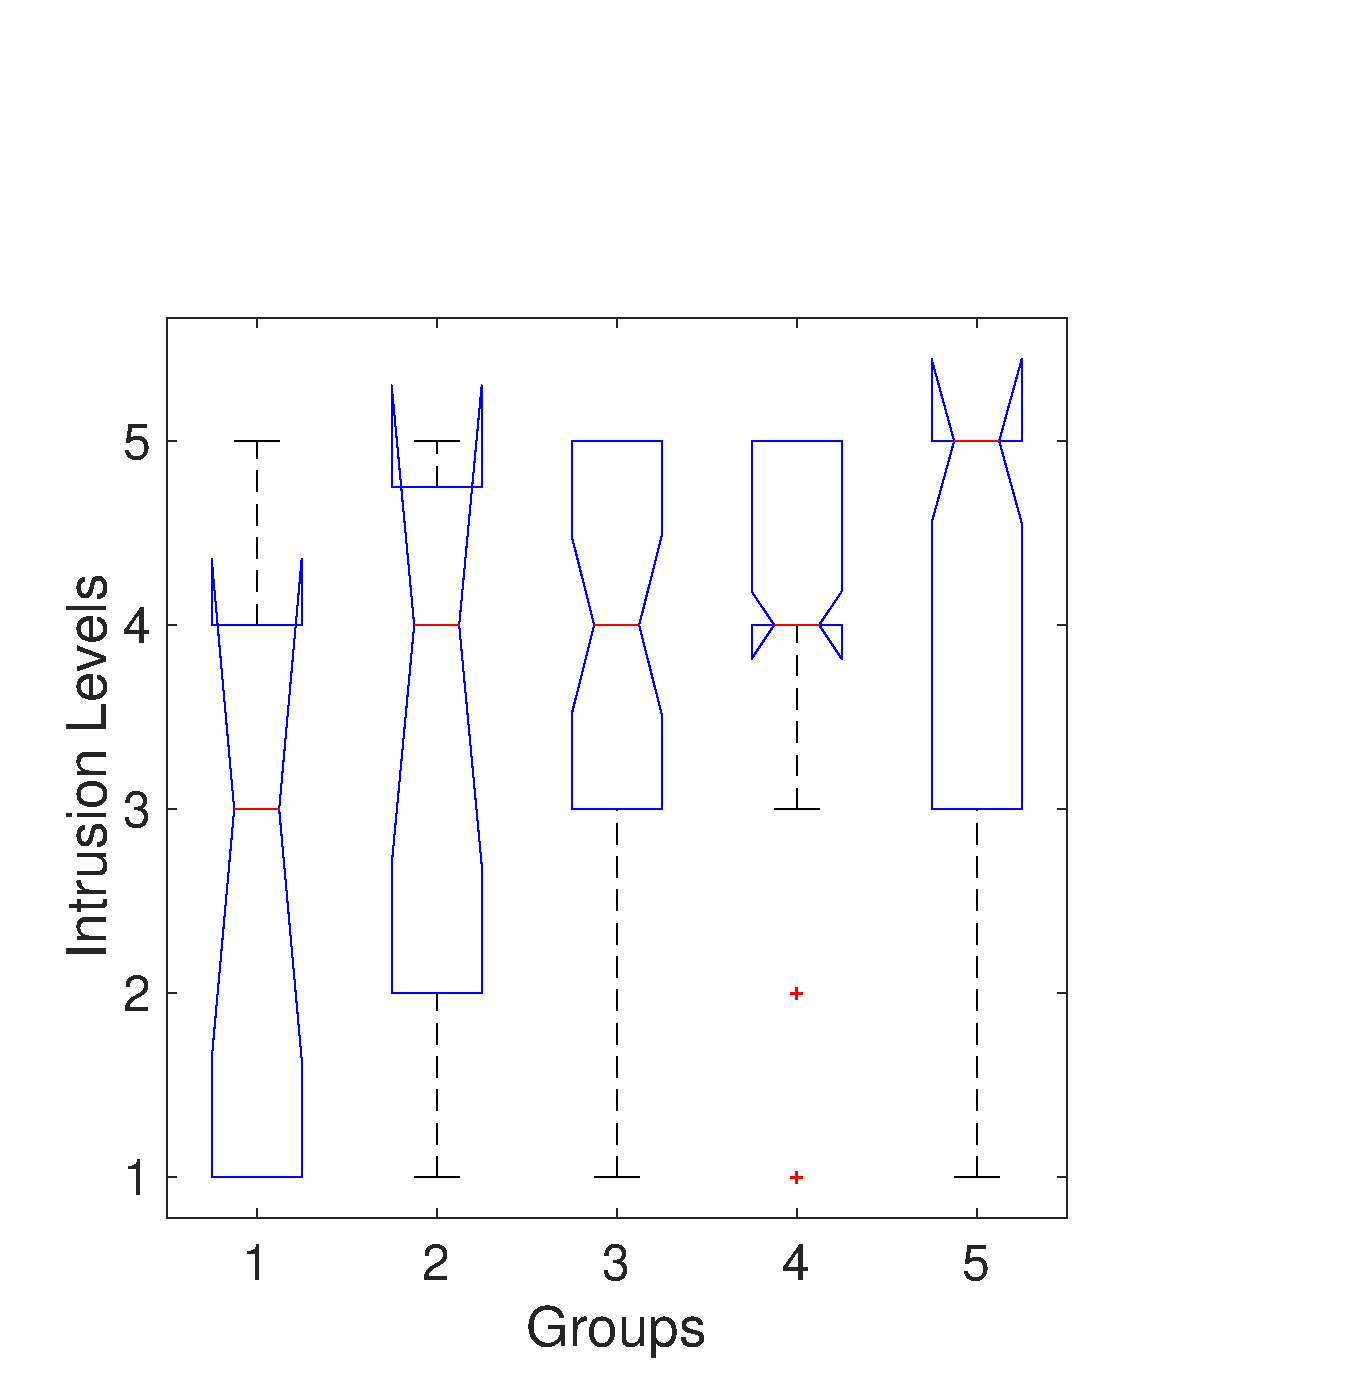
\includegraphics[width=0.4\linewidth]{./images/social_box}}\hspace{1em}
\subtop[Variance of each Group for each Stakeholder\label{fig:st2}]{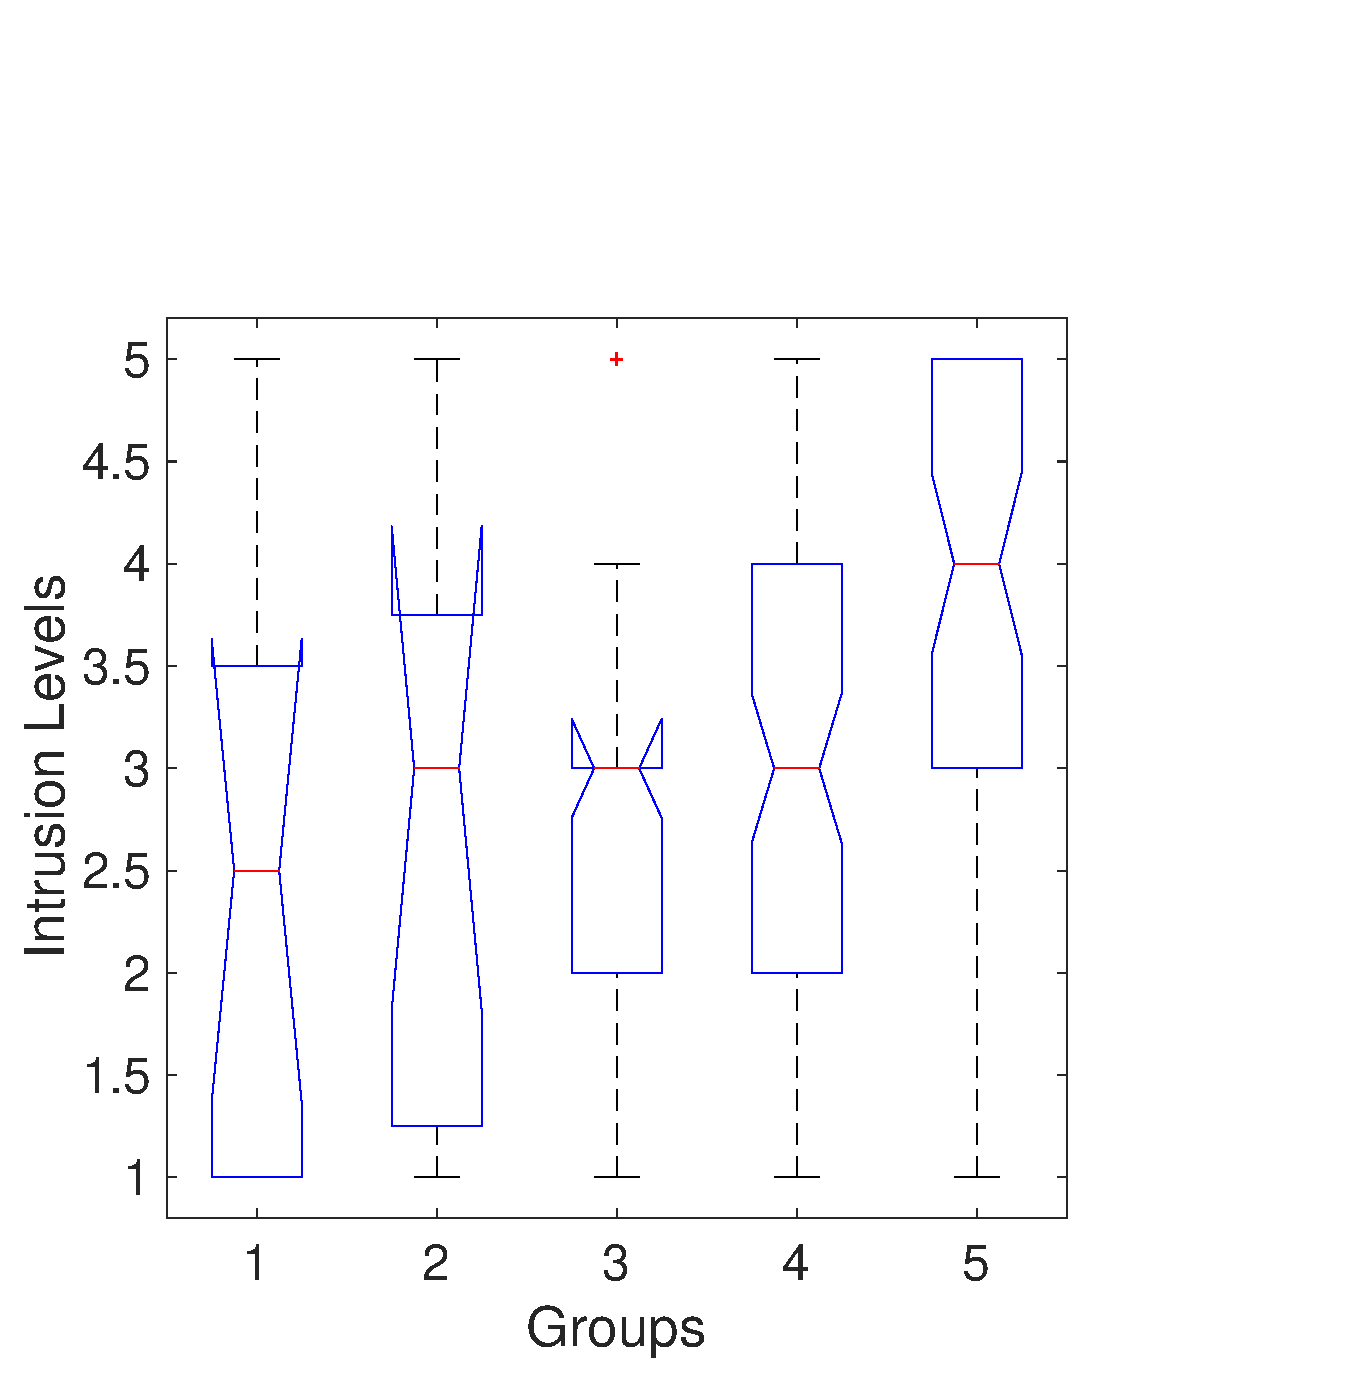
\includegraphics[width=0.4\linewidth]{./images/training_box}}\newline
\centering
\subtop[Variance of each Group for each Stakeholder\label{fig:st5}]{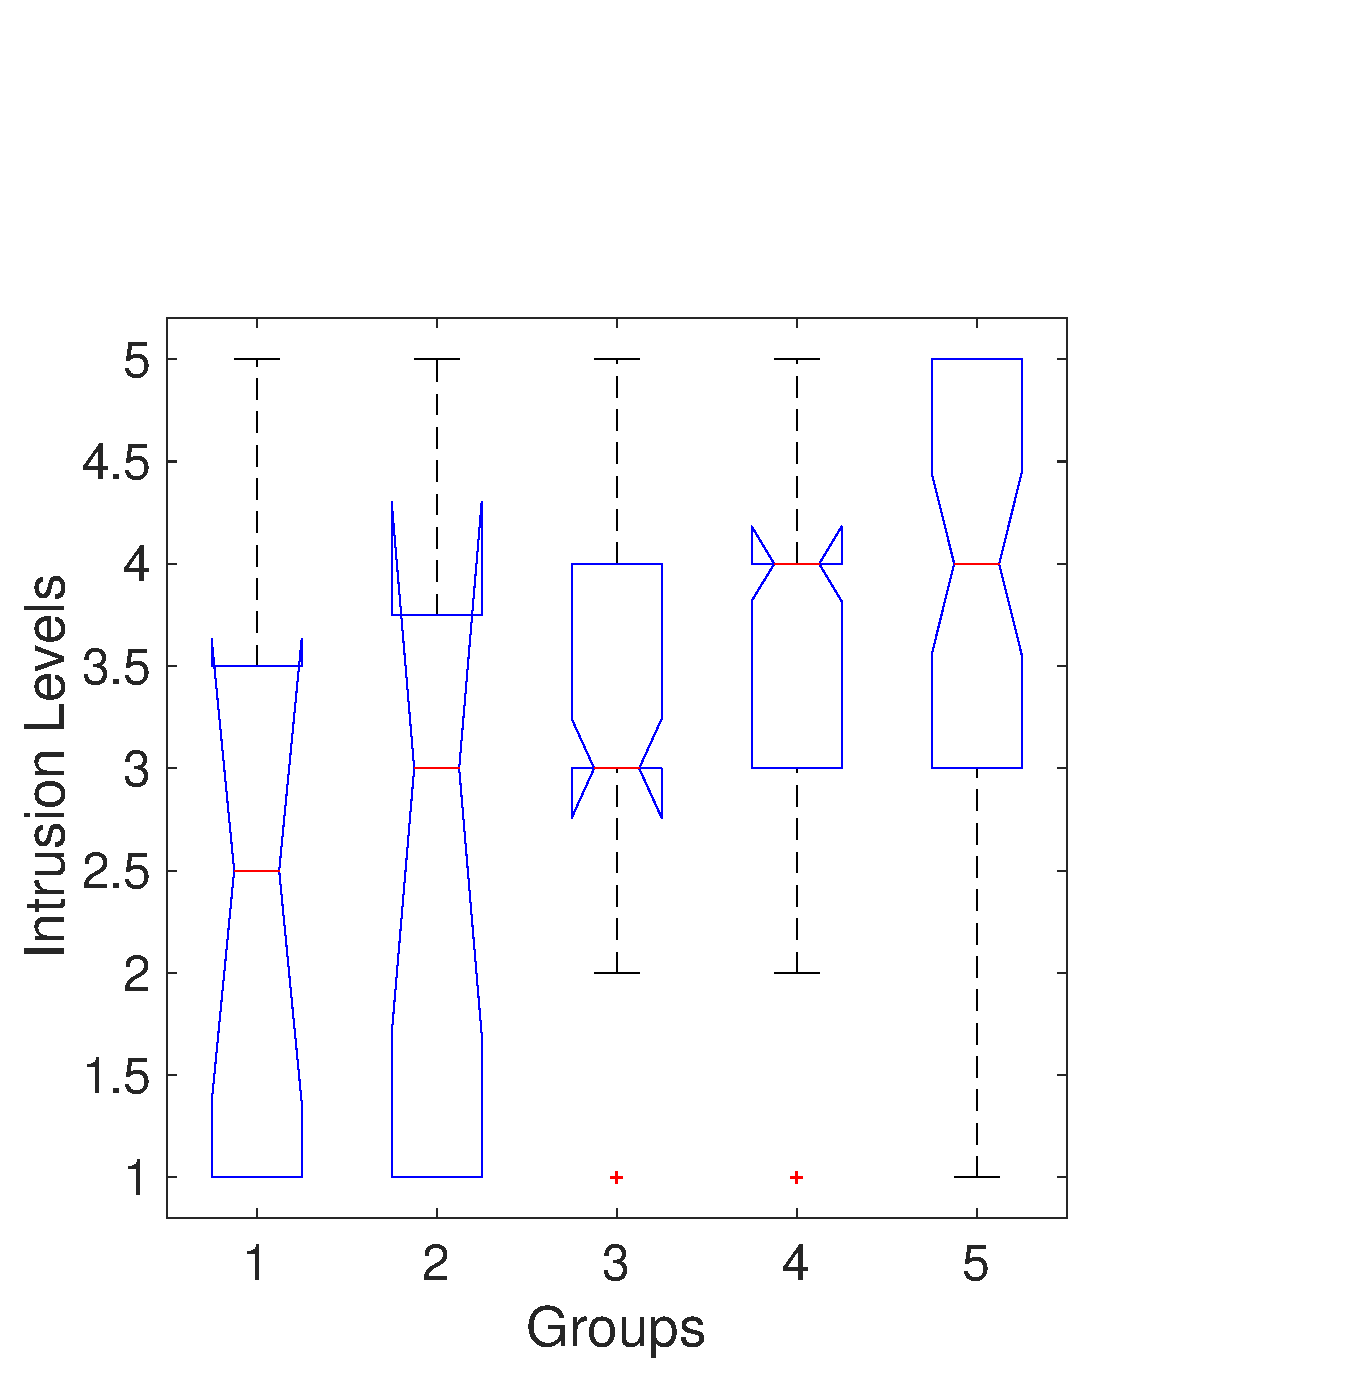
\includegraphics[width=0.4\linewidth]{./images/nav_box}}
\caption{Table Schemas}
\label{fig:st3}
\end{figure}

\section{Findings from the Experiment Data}

The social experiment described in chapter \ref{exp} is deployed using 10 participants. Out of the total of 3 days for the experiment, 3 of the participants did not answer data requests on day 2 and 3. The mobile application ran successfully on all participants phones even after being switched off. All data was successfully recorded on the server.

\begin{figure}[htp]
\subtop[all\label{fig:st5}]{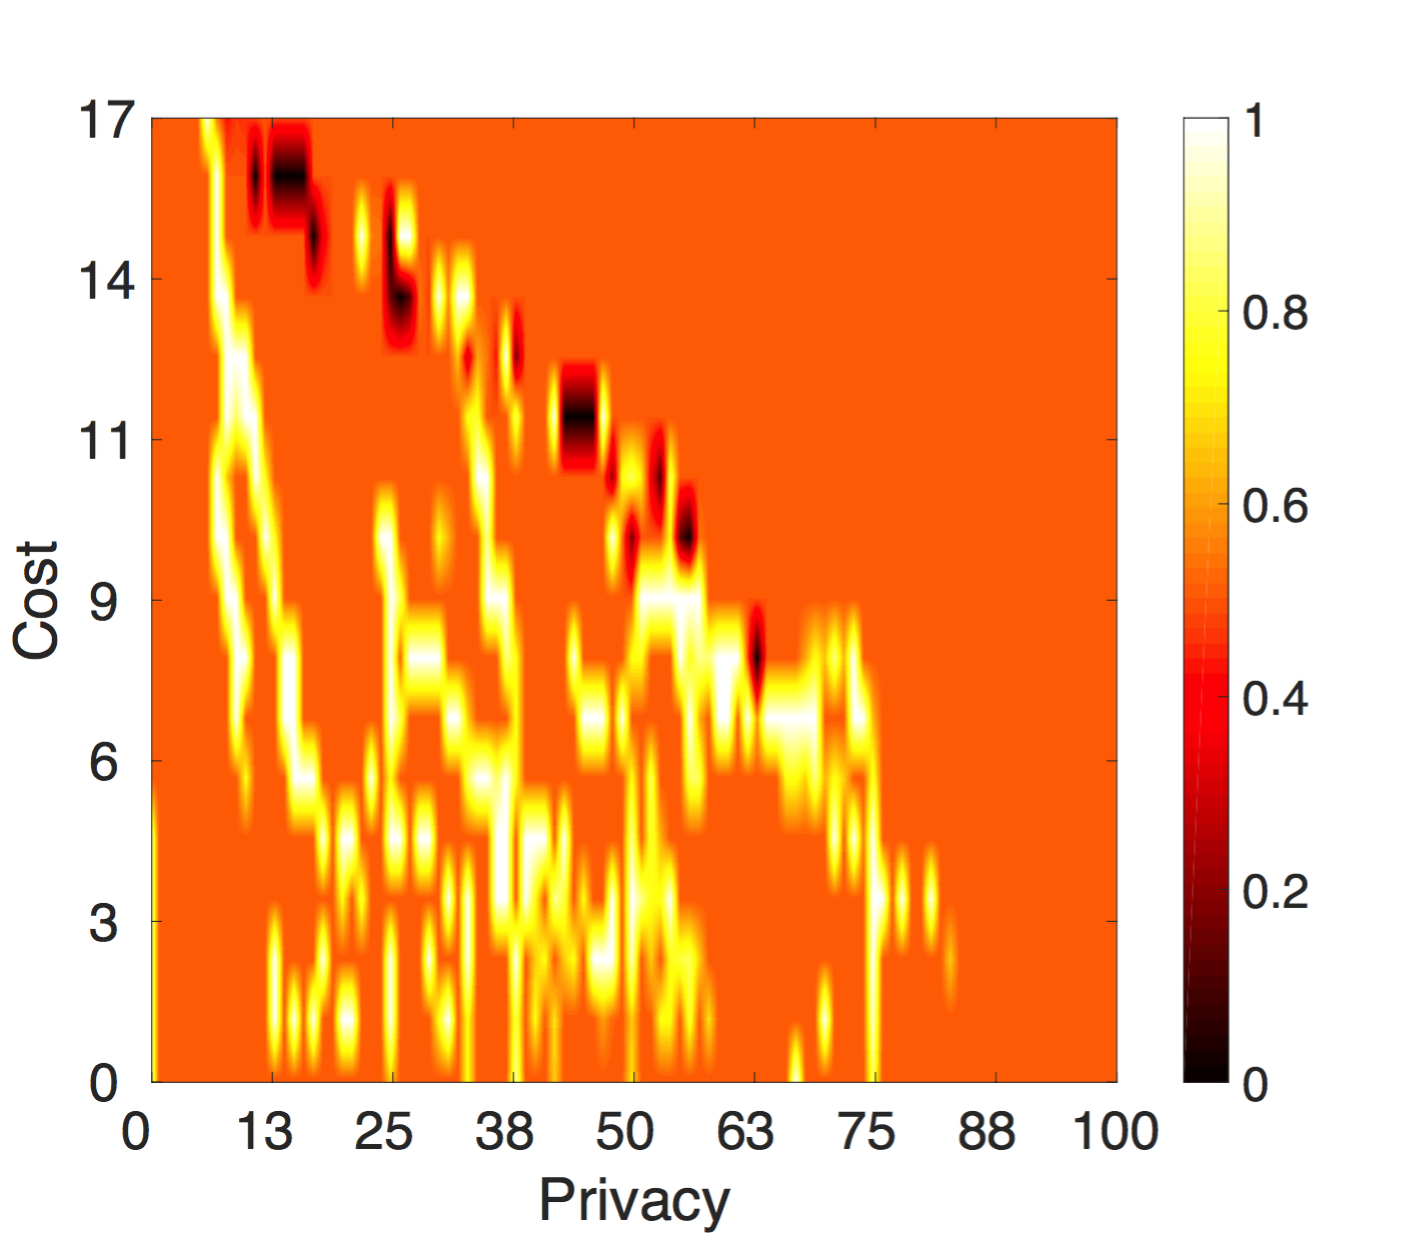
\includegraphics[width=0.4\linewidth]{./images/heatmap_all_days_privacyimprovement}}\hspace{1em}
\subtop[Variance of each Group for each Stakeholder\label{fig:st2}]{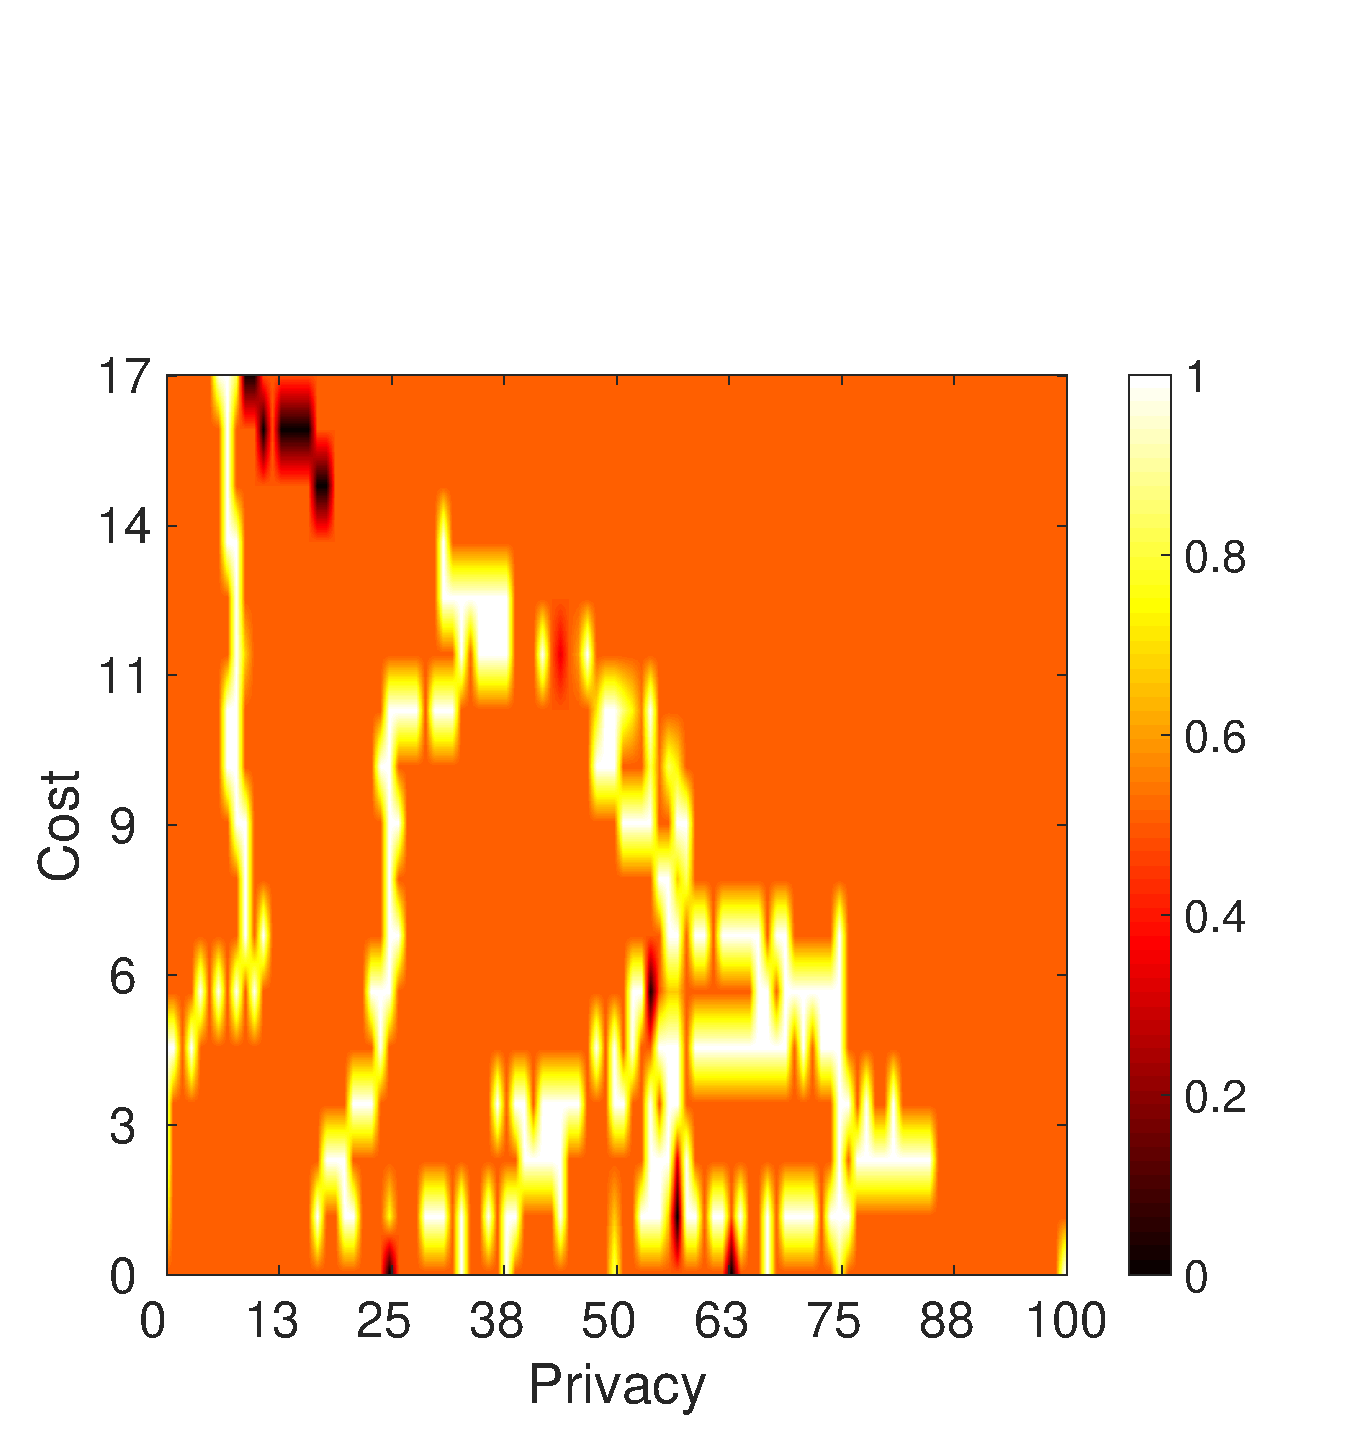
\includegraphics[width=0.4\linewidth]{./images/heatmap_all_days_button}}
\caption{Table Schemas}
\label{fig:st3}
\end{figure}

\begin{figure}[ht!]
\centering
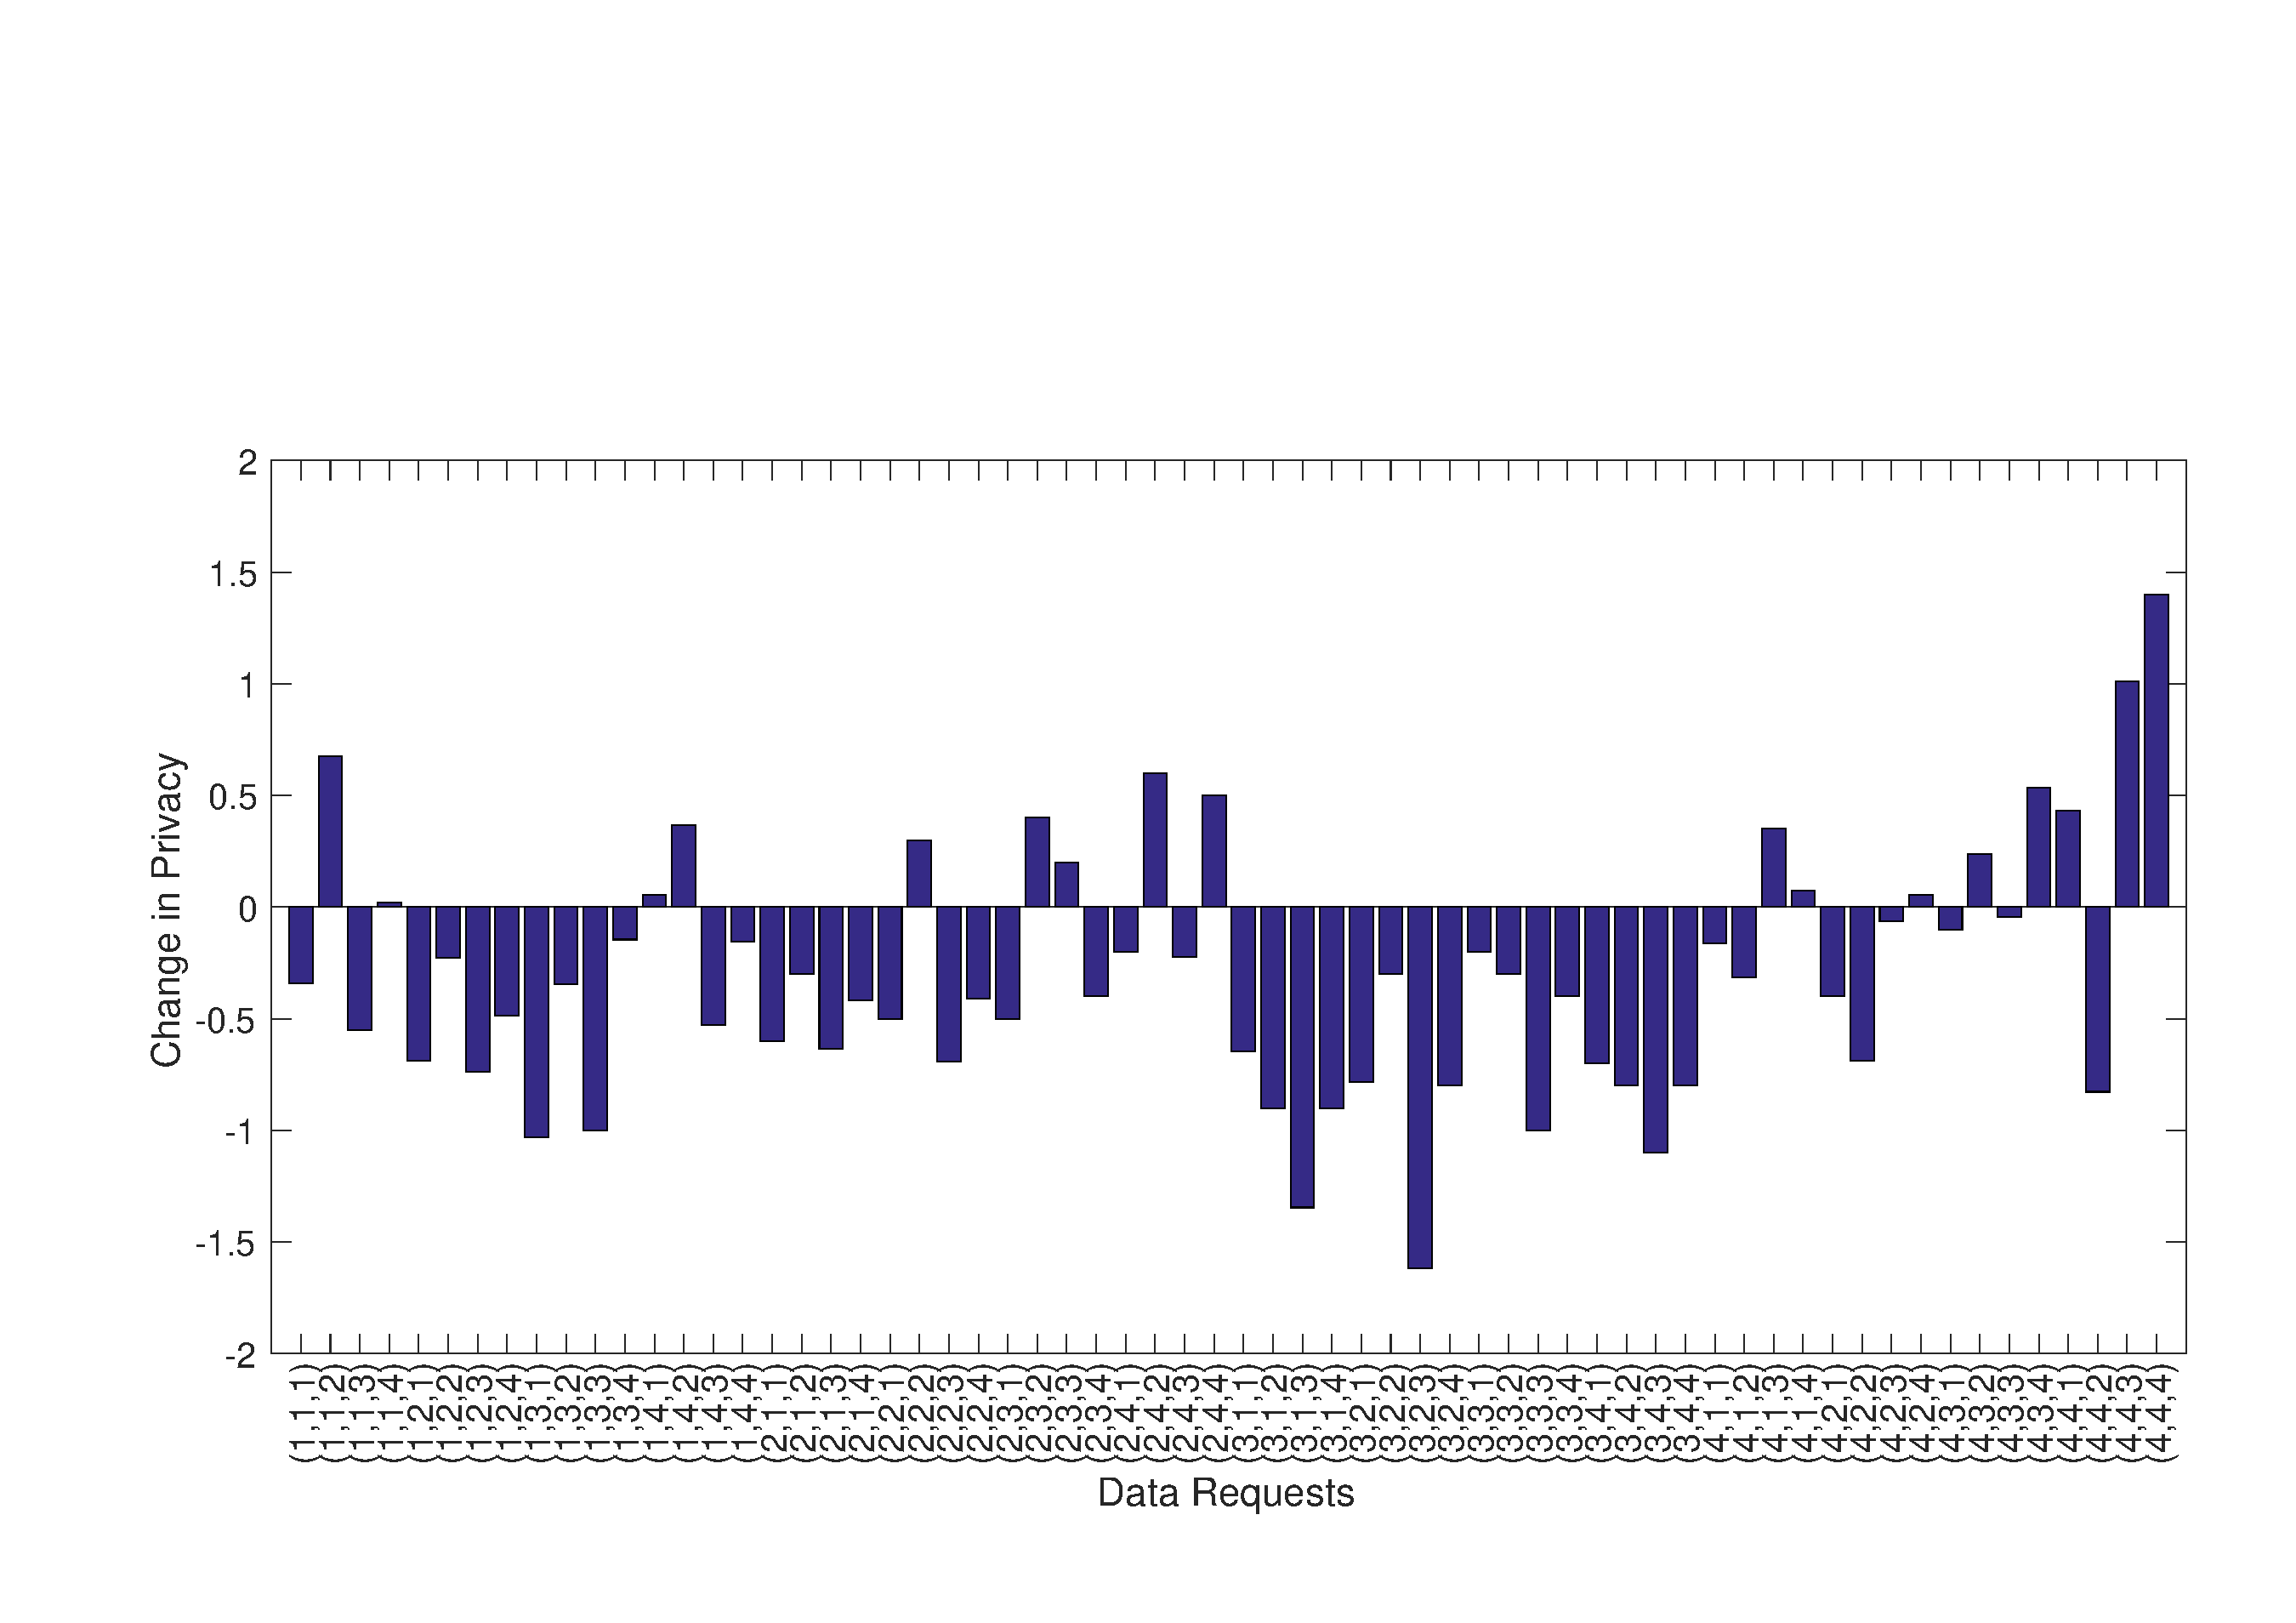
\includegraphics[width=\textwidth,keepaspectratio]{./images/day2_day1_privacy}
\caption{Applications in the Mobile Phone}
\label{fig:pre_q6}
\end{figure}

\begin{figure}[ht!]
\centering
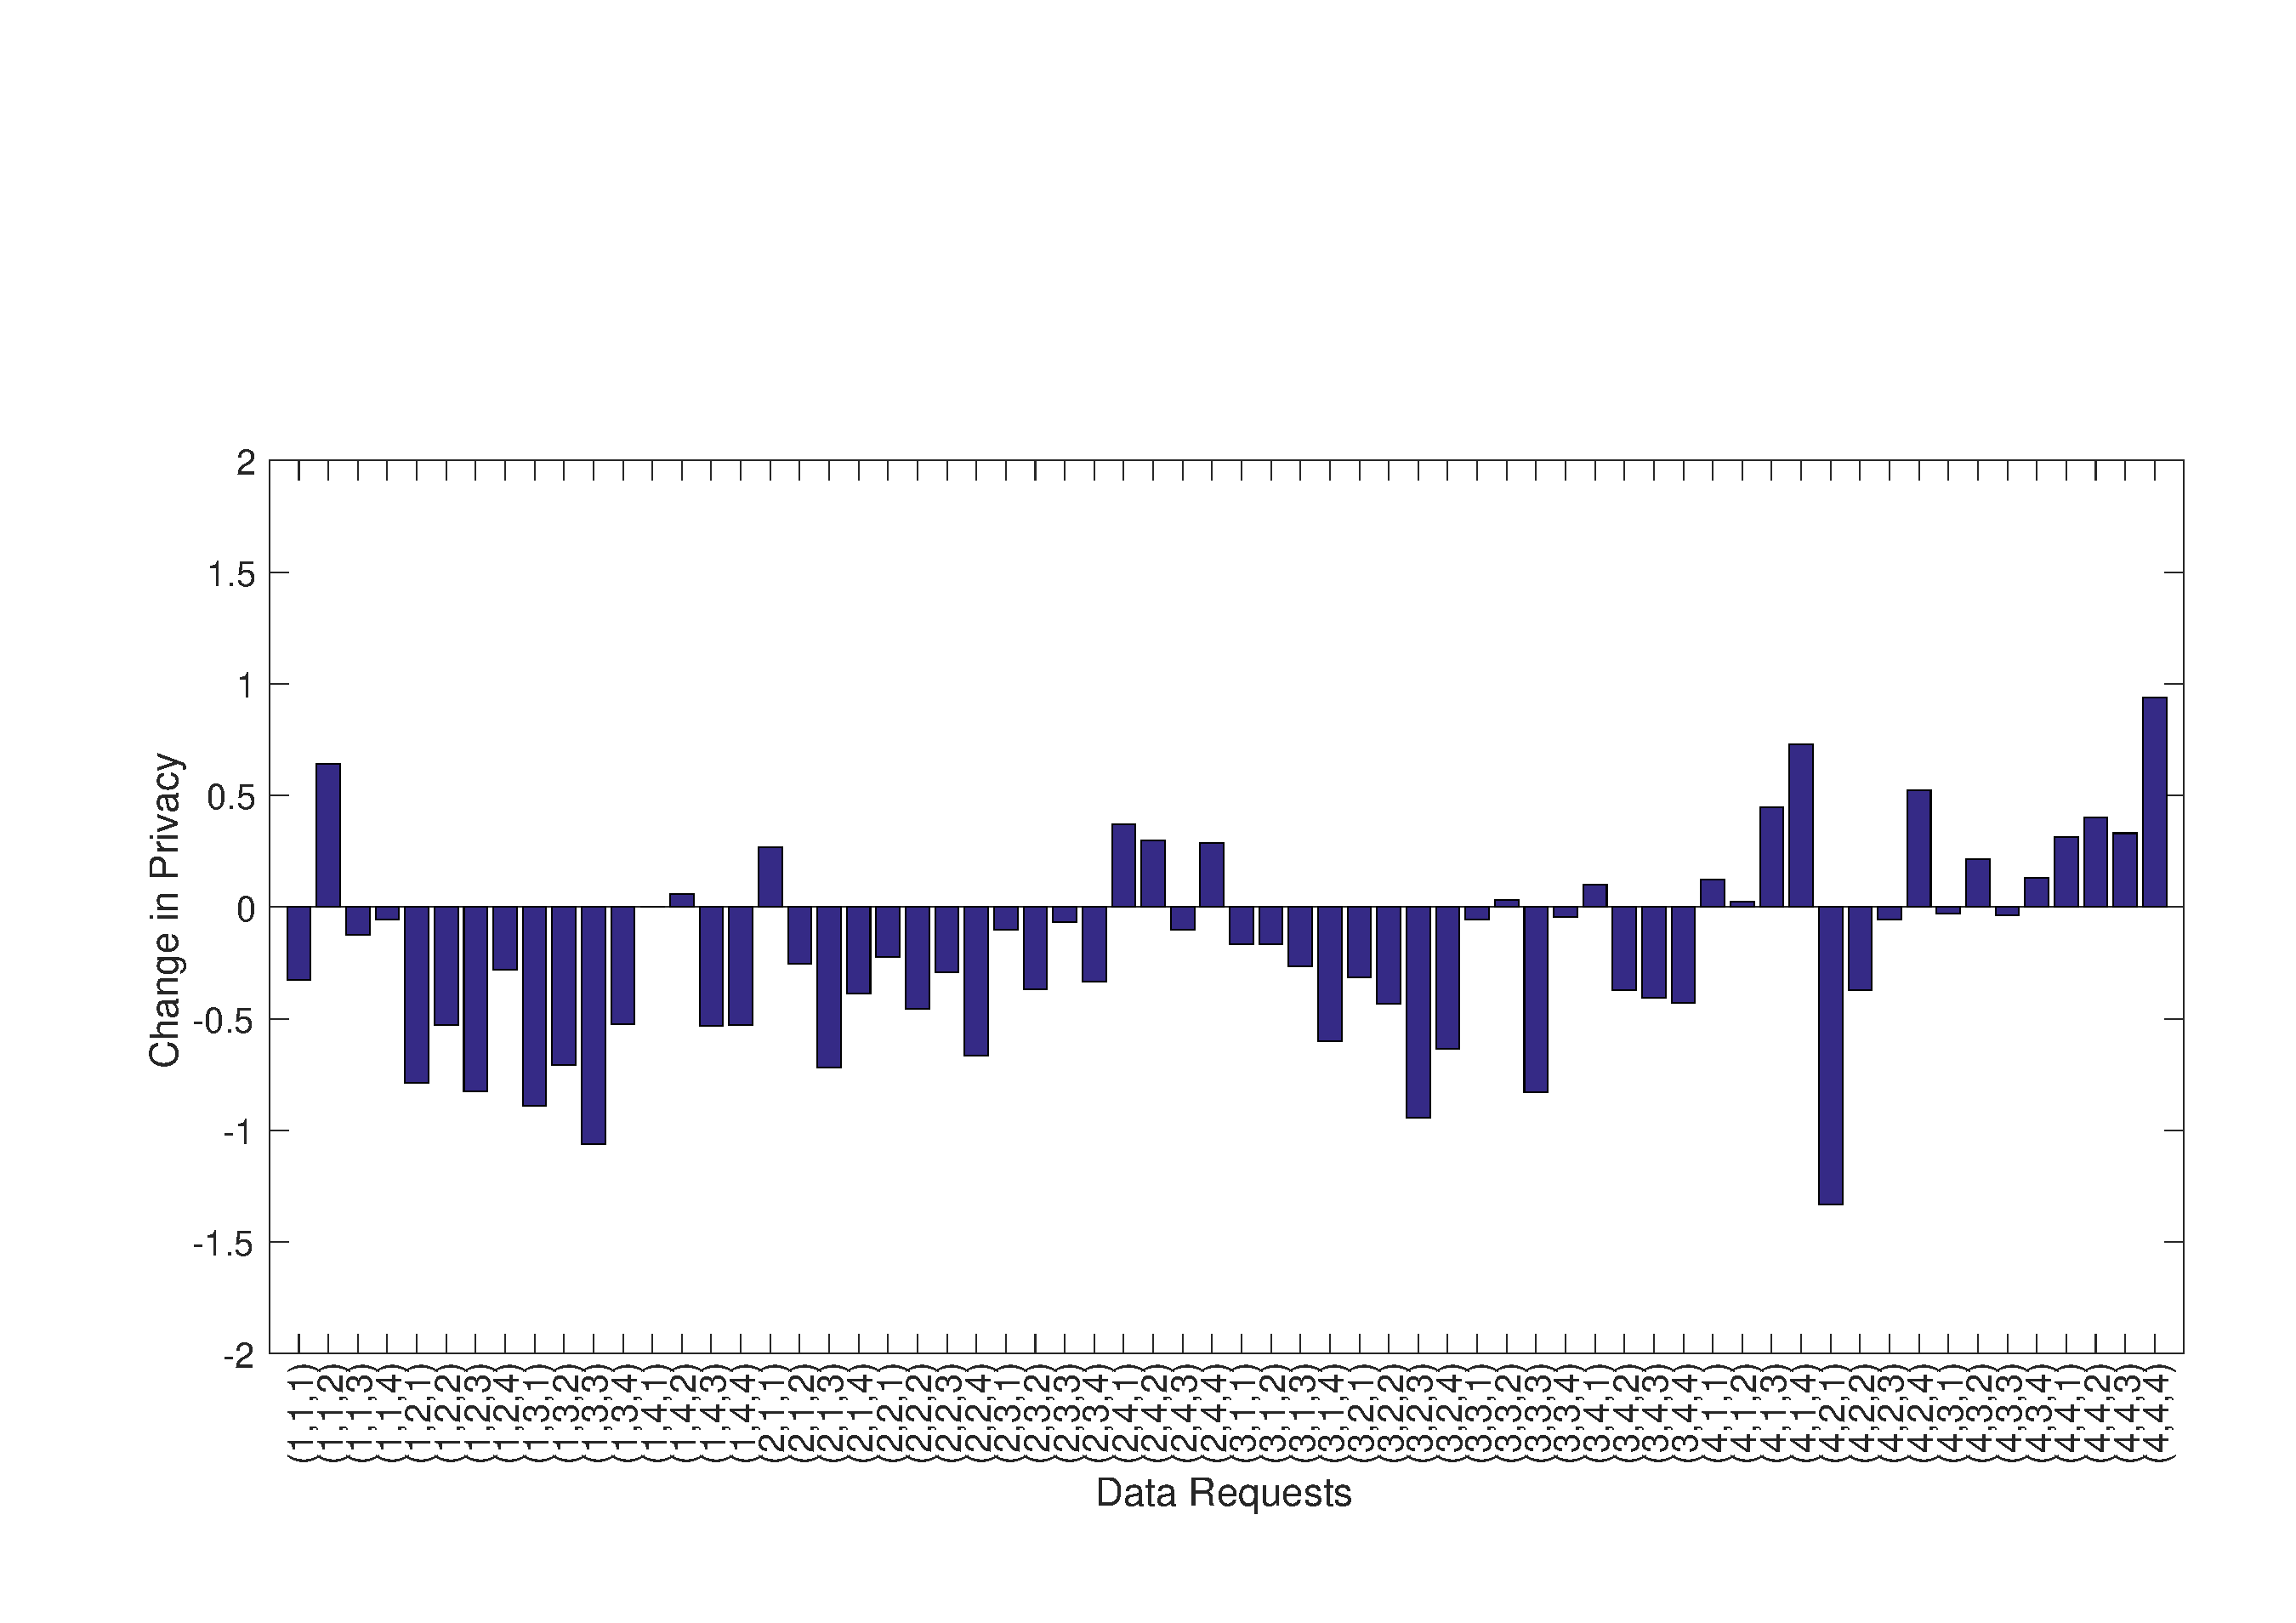
\includegraphics[width=\textwidth,keepaspectratio]{./images/day3_day1_privacy}
\caption{Applications in the Mobile Phone}
\label{fig:pre_q6}
\end{figure}





